
%----------------------------------------------------------------------------------------
%	PACKAGES AND OTHER DOCUMENT CONFIGURATIONS
%----------------------------------------------------------------------------------------

\documentclass{article}

\usepackage{fancyhdr} % Required for custom headers
\usepackage{lastpage} % Required to determine the last page for the footer
\usepackage{extramarks} % Required for headers and footers
\usepackage{graphicx} % Required to insert images
\usepackage{mathtools, bm}
\usepackage{amssymb, bm}
\usepackage{graphicx}
\usepackage{float}
\usepackage{multirow}
\usepackage[table]{xcolor}  
\usepackage{algorithm}
\usepackage[noend]{algpseudocode}

% Margins
\topmargin=-0.45in
\evensidemargin=0in
\oddsidemargin=0in
\textwidth=6.5in
\textheight=9.0in
\headsep=0.25in


\linespread{1.1} % Line spacing

% Set up the header and footer
\pagestyle{fancy}
\lhead{\hmwkAuthorName} % Top left header
\chead{\hmwkTitleComp} % Top center header
\rhead{\firstxmark} % Top right header
\lfoot{\lastxmark} % Bottom left footer
\cfoot{} % Bottom center footer
\rfoot{Page\ \thepage\ of\ \pageref{LastPage}} % Bottom right footer
\renewcommand\headrulewidth{0.4pt} % Size of the header rule
\renewcommand\footrulewidth{0.4pt} % Size of the footer rule

\setlength\parindent{0pt} % Removes all indentation from paragraphs

%----------------------------------------------------------------------------------------
%	DOCUMENT STRUCTURE COMMANDS
%	Skip this unless you know what you're doing
%----------------------------------------------------------------------------------------

% Header and footer for when a page split occurs within a problem environment


% Header and footer for when a page split occurs between problem environments
   
%----------------------------------------------------------------------------------------
%	NAME AND CLASS SECTION
%----------------------------------------------------------------------------------------
\newcommand{\logoepfl}{
  \begin{center}
    
\includegraphics[width=4cm]{img/epfl.jpg}
  \end{center}
  \vspace{0.3cm}
  \hrule
}


\newcommand{\hmwkTitle}{Decentralized Data Sharing System based on Secure Multi-Party Computation}
\newcommand{\hmwkTitleComp}{Decentralized Data Sharing System based on SMPC} % Assignment title
\newcommand{\hmwkDueDate}{Autumn 2017} % Due date
\newcommand{\hmwkClass}{IN, LCA1} % Course/class
\newcommand{\hmwkClassTime}{} % Class/lecture time
\newcommand{\hmwkClassInstructor}{D.Froelicher, J.Troncoso-Pastoriza} % Teacher/lecturer
\newcommand{\hmwkAuthorName}{Max Premi} % Your name

%----------------------------------------------------------------------------------------
%	TITLE PAGE
%----------------------------------------------------------------------------------------
\title{
\logoepfl
\vspace{2in}
\textmd{\textbf{\hmwkClass:\ \hmwkTitle}}\\
\normalsize\vspace{0.1in}\small{Due\ on\ \hmwkDueDate}\\
\vspace{0.1in}\large{\textit{\hmwkClassInstructor\ \hmwkClassTime}}
\author{\textbf{\hmwkAuthorName}}
\vspace{3in}
}

%----------------------------------------------------------------------------------------

\begin{document}

\maketitle

\newpage
\section*{Abstract}
\addcontentsline{toc}{section}{Abstract}
Unlynx and Prio are two privacy-preserving data sharing systems, with each its own way to encode/encrypt, decode/decrypt and aggregate data. While Unlynx \cite{unlynx} uses homomorphic encryption based on Elliptic Curve ElGamal and zero-knowledge proofs, Prio \cite{prio} uses Secret-sharing encoding and \textit{secret-shared non-interactive proofs}(SNIP's) to validate the data, which are claimed to perform better than classic zero-knowledge proofs \cite{proof1,proof2} in term of computation time, by relying on a time/bandwidth trade-off.\\
In this project, we compare both Unlynx and Prio in order to find a solution allying the best of both protocols.\\
We consider $m$ servers that constitute a collective authority whose goal is to verifiably compute aggregation functions over data send by $n$ data providers.\\
Several problems arise when comparing Unlynx and Prio. First, the collective authority is almost static in the first one but not in the second, and the threat model is not exactly the same as, in order to ensure correctness, it is needed to trust at least one server in Unlynx, but all in Prio. Privacy is assured if at least one server is trusted for both systems. Additionally, Unlynx's data providers have all their data encrypted, while Prio does not use homomorphic encryption, and leaves the data storage and protection to the DPs. Indeed Unlynx requires the data to be stored encrypted with a collective key, whereas Prio can process data decomposed in shares, sent by clients directly.\\
Prio also extends classic private aggregation techniques to enable collection of different kinds of statistics such as least-square regression, while Unlynx can only compute sum and count query over data.\\
The goal of this project is to :
\begin{description}
\item[$\bullet$] First implement Prio in the Unlynx framework.
\item[$\bullet$] Second to implement input validation for Unlynx.
\item[$\bullet$]{Then modify both protocols to run with the least significant difference in term of assumption and model.This will enable us to compare the protocols in a fair way.}
\item[$\bullet$] Finally, design a system that implements the best of both privacy-preserving data sharing protocols. The idea would be to combine Prio flexibility in terms of computations with the privacy and security ensured by Unlynx.\\
\end{description}

-------------------------------------------------
%	TABLE OF CONTENTS
%----------------------------------------------------------------------------------------

\newpage
\tableofcontents
\newpage


%----------------------------------------------------------------------------------------
%	BEGIN OF REPORT
%----------------------------------------------------------------------------------------

\section*{Introduction}
\addcontentsline{toc}{section}{Introduction}
Nowadays, tons of data are generated by individuals about what they do and are collected and used to compute statistics, by different parties. Even if these statistics are gathered with the goal of learning useful aggregate information about the users/population, for example, health or work statistics for a country \cite{swiss}, it might end in collecting and storing private data from data providers, which poses a serious privacy and security problem.\\
We can illustrate this example with the numerous problem of Cloud leaks/breaches that happened several times in the past years \cite{pentagon}, or the divulgation of sensitive health data such as susceptibility to contract diseases, that can be used against one individual \cite{sell}. They might even be disclosed, sold for profit \cite{sold} or be used by agencies for targeting and mass surveillance goals, as some countries do not have highly regulated Data privacy laws e.g., the U.S \cite{law}, meaning they are less restricted to use these data.\\
The need to collect data and to share them in a privacy-preserving way has become crucial in this context, and a lot of research has been done on this topic.\\
The techniques are developed through research efforts at prominent research groups \cite{unlynx,prio}, and some companies have already implemented some of these mechanisms in their commercial products \cite{apple}.\\
First, systems that use "Randomize response for differential privacy" \cite{randomized} were developed. It relies on a method that changes a value with probability $p < 0.5$.
When aggregating a large number of noisy values, the aggregation is still a good estimation of the real values. This technique is well scalable and performs nicely, but ensures only \textit{weak privacy}.\\
So encryption-based systems were developed to solve this problem.
However, by gaining \textit{privacy}, these protocols sacrifice \textit{robustness} and \textit{scalability}, which are two important aspects to keep in mind while designing a decentralized system. Privacy is necessary so that no leak in the sensitive data happens, and robustness characterizes the correctness of the computation. The trade-off between both should be reasonable, as we do not want any data to be leaked, and the server has to correctly compute under given assumptions and models.\\
These difficulties lead to the use of legal agreements rather than technical solutions, as only a few technically-enforced privacy conscious systems have been deployed in the real world. This agreement is not a robust solution for several reasons.\\
One of them is centralization. Centralized systems are still widely used \cite{dyadic, centralized} because they are way simpler but they rely on a trusted third party, which represents a single point of failure in the system.\\
Another reason is that data providers have begun to realize the importance and value of their own data.
This is why decentralized systems are becoming more popular, and desirable. We can also illustrate the growth of decentralized systems with the rise of Cryptocurrencies such as Bitcoin \cite{bitcoin}. Prio and Unlynx are both distributed protocols following the same decentralized trust trend.\\
In this paper, we present the implementation of Prio into Unlynx's framework, an implementation of an improved Unlynx that includes input validation and a theoretical comparison and discussion for future possible new systems that combine, if possible, the best part of each approach.
	
\section*{Contributions}
\addcontentsline{toc}{section}{Contributions}
In this paper, the following contributions are made:\\
- An implementation of Prio Secred Shared Non-Interactive Proofs (SNIPs) system in Unlynx's framework, represented as two new protocols, and a new service. It includes the input validation and the aggregation. It also contains the different data types supported by Prio.\\

- The implementation of a novel proof for input range validation for Elliptic Curve ElGamal, using pairings on a specific Elliptic Curve. This allows the server to exclude faulty data sent by possible malicious clients. The range to check is $[0,u^l]$ with $u,l$ taking arbitrary values.\\

- An evaluation of both protocols in terms of privacy and efficiency, with a comparison with the most similar settings. Then, we provide some guidelines on how to  combine the advantages of both systems and a description of future work.


\section*{Background}
\addcontentsline{toc}{section}{Background}
This section introduces some fundamental concepts used throughout the rest of the report. \textit{Collective Authority} that is the base of both system functionality. \textit{ElGamal encryption} is used in Unlynx to ensure privacy, while \textit{arithmetic circuits} are used by Prio to ensure correctness of data.\\
\textit{Beaver's triple} are used in Prio's multi-party computation part, and \textit{Affine-aggregatable functions} are used to enable different aggregation functions. 
Finally, Bilinear pairing over Elliptic Curve is used in Unlynx's input range validation.\\

\subsection*{Collective Authority}
Nowadays, applications and systems rely on third-party authorities to provide security services. For example the creation of certificates to prove ownership of a public key. A collective authority is a set of $m$  servers that are deployed in a decentralized and distributed way, to support a given number of protocols.\\
Each of them possesses a private-public key pair $(k_i,K_i)$, where $K_i = k_i B$ with $k_i$ a scalar and $K_i$ a point in a given Elliptic Curve. This authority constructs a public key $K = \sum_{i=1}^{m}{K_i}$ which is the sum of all the server's public keys. To decrypt a message, each server $i$ partially decrypts a message encrypted using $k_{i}$. Thus the collective authority key provides strongest link security, as no intermediate can decrypt the data without the contribution of all the servers.

\subsection*{ElGamal Encryption}
All the involved scalars belong to a field $\mathbb{Z}_p$.\\
For Unlynx, data are encrypted by using Elliptic Curve ElGamal, more precisely, $P$ is a public key, $x$ is a message mapped to a point and $B$ is a base point on the curve $\gamma$. The encryption is the following, with $r$ a random nonce:\\
$E_P(x) = (rB,x+rP)$. The additive homomorphic property states that $\alpha E_P(x_1) + \beta E_P(x_2) = E_P(\alpha x_1+ \beta x_2)$\\
To decrypt, the owner of the private key $p$ satisfying $P = pB$ multiplies $rB$ and $p$ to get $rP$ and substracts it from $x + rP$ to recover $x$.\\

\subsection*{Arithmetic Circuits}
An arithmetic circuit $C$ over a finite field $\mathbb{F}$ takes as input a vector $x = (x^{(1)},...,x^{(L)}) \in \mathbb{F}^L $. It is represented as an acyclic graph with each vertex either being an \textit{input}, \textit{output} or a \textit{gate}.\\
There are only two types of gates, addition and multiplication, all in finite field $\mathbb{F}$.\\
A circuit $C$ is just a mapping $\mathbb{F}^L \rightarrow \mathbb{F}$, as evaluating is a walk through the circuit from inputs to outputs.

\subsection*{Beaver's MPC triples}
A Beaver triple is defined as follows:\\
$(a,b,c) \in \mathbb{F}^3$, chosen at random with the constraint that $a \cdot b = c$.\\
As we use it in a multiparty computation context, each server $i$ holds a share $([a]_i , [b]_i , [c]_i) \in \mathbb{F}^3$.\\
Using these shares, the goal is to multiply two numbers $x$ and $y$ without leaking anything about them. In Prio the goal is to multiply shares $[x]_i$ and $[y]_i$.\\
To do so, the following values are computed:
$$[d]_i = [x]_i -[a]_i  \quad  ;  \quad  [e]_i = [y]_i - [b]_i$$ 
Then from this shares, each server can compute $d$ and $e$ and compute this formula:\\
$$\sigma_i = de \cdot m^{-1} + d[b]_i +e[a]_i + [c]_i$$
The sum of these shares yields:

\begin{equation}
\begin{split}
& \sum_{i} \sigma_i = \sum_{i}{(de/m +d[b]_i + e[a]_i + [c]_i)}\\
 & = de +db +ea + c\\
 & = (x-a)(y-b)+ (x-a)b + (y-b)a + c\\
 & = (x-a)y + (y-b)a + c\\
 & = xy -ab + c\\
 & = xy\\
\end{split}
\end{equation}
As $\sum_{i} \sigma_i = xy$, it implies that $\sigma_i = [xy]_i$ 

\subsection*{Affine-aggregatable encodings (AFEs) functions}
\label{afe}
Given the fact that each data provider $i$ holds a value $x_i \in D$, and the servers have an aggregation function $f : D^n \rightarrow A$, whose range is a set of aggregates $A$, an AFE gives an efficient way to encode data such that it is possible to compute the value of the aggregation function $f(x_1,...,x_n)$ given only the \textit{sum of the encodings} $x_1,....,x_n$. This technique enables the computation of min, max, set intersection and others by doing only aggregations at the servers.\\
It comprises three Algorithm (Encode, Valid, Decode) defined in a field $\mathbb{F}$ and two integers $k' \leq k$\\
\begin{itemize}
\item \textbf{Encode($x$)}: maps an input $x \in D$ to its encoding in $\mathbb{F}^k$
\item \textbf{Valid($y$)}: returns true if and only if $y$ is a valid encoding of some item in $D$
\item \textbf{Decode($\sigma$)}: $\sigma = \sum_{i=1}^{n}{Trunc_{k'}(Encode(x_i))} \in \mathbb{F}^{k'}$ is the input (Trunc takes the $k' \leq k$ components of the encoding), and it outputs the aggregation result $f(x_1,...,x_n)$.
\end{itemize}

\subsection*{Bilinear pairings over Elliptic Curve}
Let $G_1$ and $G_T$ be two additive groups of points of an elliptic curve $G$ over a field $\mathbb{F}$ of order $n$ and with identity $O$. Then the mapping $e: G_1 \times G_1 \rightarrow G_T$ satisfies the following conditions:\\
For all $R,S \in G_1$ and $x \in \mathbb{F}$, $e(R,S)(x) = e(Rx,S) = e(R,Sx)$\\
For $B$ the base point, $e(B,B) \neq O$, and the mapping is efficiently computable.


\section{Unlynx System}
This section presents Unlynx \cite{unlynx} system in general. It goes through the model design, the assumptions made about the parties taking part in the general protocol, and a detailed pipeline of which protocols are executed to achieve the goal of the system. It also describes briefly describes the proofs done at each step.\\

\subsection{System Model}
\begin{figure}[H]
\centering
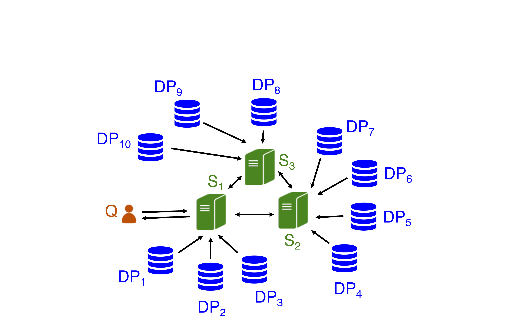
\includegraphics[scale=0.8]{img/UnlynxFunc.png}
\end{figure}
Unlynx is a privacy-preserving data sharing system developed by LCA1 \cite{lca} in collaboration with DeDiS \cite{dedis}.\\
It consists of a collective authority (CA) formed by $m$ servers $S_1,...,S_m$, and $n$ data providers $DP_1,...DP_n$ containing sensitive data, encrypted using EC ElGamal by following the scheme described in the \textbf{Background} Section. These DPs combined represent a distributed database that is used to answer queries made by a querier $Q$. The querier and DPs choose one server of the CA to communicate with and can change this choice at any given time.\\
\textbf{Functionality}: Unlynx should permit SQL queries of the form SELECT SUM(*)/COUNT(*) FROM DP,.... WHERE * AND/OR GROUP BY *, with any number of * clauses, but only equality ones.\\
\textbf{Privacy and Robustness}: Both are assured if at least one server is trusted, as we use the fact that it is allowed to publish ciphertexts and their aggregation to show that the computation at the servers is actually correct. It leaks nothing as all data are encrypted.\\
Also, the data are never decrypted and a key switch protocol is used to sequentially change the encryption key from the CA's public one to the querier's $Q$ public one. This way, the privacy of data is ensured, as to break the protocol, all servers in the CA would have to collude, which is not possible with the actual threat model, described in the next section.

\subsection{Threat Model}
\textbf{Collective authority servers} It is assumed an Anytrust model \cite{anytrust}. It does not require any particular server to be trusted or to be honest-but-curious. Whenever one of the servers is not malicious, functionality, security, and privacy are guaranteed.\\
\textbf{Data providers} are assumed to be honest-but-curious. The system does not protect against malicious DPs sending false information, but a solution will be discussed  in Section \textbf{Input range validation for Elliptic Curve ElGamal}.\\
\textbf{Queriers} are assumed to be malicious, and can collude between themselves or with a subset of the CA servers.\\
It is also assumed that all network communication is encrypted and authenticated, by using a protocol like TLS for example.

\subsection{Pipeline and proof}
The protocol starts when a querier wants to retrieve some information about sensitive data. It sends the query to one of the servers of the CA. Upon receiving the request, the server broadcasts this query to the other servers in the collective authority.\\
From here the data are privately and securely processed by the CA, before sending back the result to the querier, encrypted the public key of the querier. During all the steps of the protocol, the servers will never see the data in clear.\\
The pipeline comprises the following secure protocols: Encryption, Verifiable Shuffle, Distributed Deterministic Tag, Collective Aggregation, Distributed Results Obfuscation and finally Key Switch. At the end of this pipeline, the querier gets the data and can decrypt them to get the aggregate statistics he asked for, without any server seeing the data in clear, or knowing from which data provider the data are from.\\
The steps of the protocol are not detailed in this report, but some of them are used for comparison with Prio and are discussed in the \textbf{Implementation} section.
\begin{figure}[h]
\centering
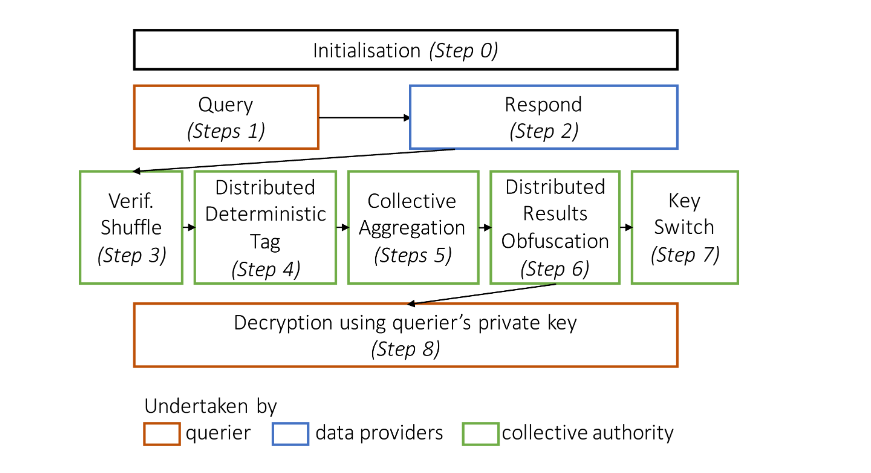
\includegraphics[scale=0.5]{img/unlynxPip.png}
\caption{Unlynx query processing pipeline}
\end{figure}
\\
\textbf{Proofs}: Zero-knowledge proofs are used to validate the correctness of inputs and computations without disclosing the involved secrets and private inputs.\\

To illustrate one of them, while doing the aggregation phase, the server publishes the ciphertexts and the result of their aggregation. As the data is encrypted using Elliptic curve ElGamal, it leaks nothing about the data.\\
However, one of the problems in Unlynx is that it provides no input range proof for data coming from the data providers, meaning the DPs can send false, forged or incorrect datae, e.g., very big or very small quantities and as data are encrypted the servers have no way to directly check the actual value sent. This makes the whole result and computation invalid if we assume malicious DPs, and this is why in the basic Threat Model, data providers are assumed honest-but-curious. This input validation proof is implemented and described in the following section.  It is an adaptation, completely novel, developed for the project, taken from the references \cite{range}, and adapted to be non-interactive and usable with Elliptic Curve ElGamal encryption.\\

\subsection{Input range validation for Elliptic Curve ElGamal}

A problem with data encryption is that we can not be sure if received data are correct. An example would be an aggregation where input values should be in the range $[0,100)$. In the current system's settings, if a malicious data provider wants to send a value of $15000$ to falsify information, it can do it. This section presents an  interactive algorithm based on a classic ElGamal input range validation \cite{range}, and we discuss its novel non-interactive form in the \textbf{Implementation} section.\\
We need to define some parameters before jumping into the algorithm. A scalar in the elliptic curve is defined over the field $\mathbb{Z}_p$. Also, we denote $e()$ the bilinear map that is described in the Background section.\\
This is the algorithm that allows checking the validity of a secret $\sigma$ in a range $ [0,u^l]$. The algorithm can be adapted to check any range $[a,b]$.\\


\begin{algorithm}[H]
\caption{Interactive Range Validation}\label{euclid}
\begin{algorithmic}[1]

\State In the algorithm, the terms \textit{Prover} and \textit{Verifier} are used. In our case it should be clear that the prover is the data provider and the verifier the CA containing all the servers.\\
\State \textbf{Common Input:} $B$ Elliptic Curve base,  $P$ a public key, $ u, l$ , 2 integers and $C$ commitment.
\State \textbf{Prover Input:} 
$\sigma,$ the value to encode mapped to a point in the EC and $r$ a scalar in the EC such that $C = \sigma + Pr$, with $\sigma \in [0,u^l)$\\
\State  \textbf{P $\leftarrow$ V}: verifiers pick $x_i \in \mathbb{Z}_p$ define $y_i \gets Bx_i$\\
and send to the prover $A_{i,j} \gets B(x_i+j)^{-1}$ $ \forall j \in \mathbb{Z}_u$ and $ i \in \{0,...,m\}$\\
\State \textbf{P $\rightarrow$ V} Then prover encodes the signature of the value to check in base $u$ with randomly picked $v_j$.\\
So $\forall j \in \mathbb{Z}_l $ such that $ \sigma = \sum_{j}{\sigma_j u^j}$, it picks $v_j \in \mathbb{Z}_p$ and sends $V_{i,j} = A_{i,\sigma_j}v_j$ back to server $i$\\
\State \textbf{P $\rightarrow$ V}: prover picks 3 values $s_j,t_j,m_j \in \mathbb{Z}_p $, $\forall j \in \mathbb{Z}_l$ and sends to each server $i$:\\
$a_{i,j} \gets e(V_{i,j},B)(-s_j)+e(B,B)(t_j)$\\
$D \gets \sum_{j}{(u^j s_j + Pm_j)}$\\
\State \textbf{P $\leftarrow$ V} Verifier sends a random challenge $c \in \mathbb{Z}_p$\\
\State \textbf{P $\rightarrow$ V} Prover sends the following value for Verifiers to compute verification.\\
$ \forall j \in \mathbb{Z}_l$, $Z_{\sigma_j} \gets s_j-\sigma_j c$ and $Z_{v_j} \gets t_j-v_j c$\\
$Z_r = m -rc $, where $m = \sum_{j}{m_j}$\\
\State \textbf{Verifier} $i$ checks that $D = Cc + PZ_r + \sum_{j}{(Bu^j Z_{\sigma_j}}) $\\
$a_{i,j} = e(V_{i,j},y)c + e(V_{i,j},B)(-Z_{\sigma_j}) + e(B,B)(Z_{v_j})$, $\forall j \in \mathbb{Z}_l$
\end{algorithmic}
\end{algorithm}

This algorithm has been adapted from the paper on Set membership over ElGamal \cite{range}, used with classic ElGamal encryption. The prover needs to compute $5l$ point multiplications in the protocol.\\
The completness follows from inspection, while soundness follows from the unforgeability of the Boneh-Boyen signature \cite{boneh}.\\
In addition, a zero-knowledge proof must satisfy another property in addition to completeness and soundness. It is that if the statement is true, no verifier learns anything else than the fact that the statement is true.
This can be showed by a \textit{simulator}, that given only the statement to be proved and no access to the prover, it can produce a transcript that "looks like" an interaction between a prover and the cheating verifier.\\
The simulator \textit{Sim} is constructed as follows for a verifier V:\\

\begin{algorithmic}
\State 1. \textit{Sim} retrieves $y,\{A_i\}$ from V with $i \in \mathbb{Z}_u$.
\State 2. \textit{Sim} chooses $\sigma \in [0,u^l)$, $v_j \in \mathbb{Z}_p$ and sends $V_j \gets A_{\sigma_j} v_j$, for each $\sigma_j$ such that $\sigma = \sum_{j}{\sigma_j u^j}$ with $ j \in \mathbb{Z}_l$
\State 3. \textit{Sim} chooses $s_j,t_j,m_j \in \mathbb{Z}_p$ for each $V_j$ and sends $a_j \gets e(V_j,B)(-s_j) + e(B,B)(t_j)$ for each $j$ and $D \gets \sum_{j}{(u^j s_j + Pm_j)}$
\State 4. \textit{Sim} receives $c$ from V.
\State 5. Eventually \textit{Sim} computes for each $j$, $Z_{\sigma_j} =s_j - \sigma_j c$, $Z_{v_j} = t_j - v_j c$ and also $Z_r = m - rc$, where m is the sum of $m_j$, to V.  
\end{algorithmic}

\subsubsection*{Arbitrary Range :}
To handle an arbitrary range $[a,b]$, the prover needs to show that $\sigma \in [a,a+u^l]$ AND $ \sigma \in [b-u^l,b]$, this leads to the following formula:\\
\begin{gather*}
 \sigma \in [b-u^l,b] \Longleftrightarrow   \sigma - b + u^l \in [0,u^l) \\
\sigma \in [a,a+u^l] \Longleftrightarrow   \sigma - a  \in [0,u^l)\\
\end{gather*}
The only needed modification in the algorithm is the verifier's check which is now:
\begin{gather*}
D = Cc+B(-B+u^l)+P(Z_r)+\sum_j{B(Z_{\sigma_j})}\\
D= Cc+B(-A)+P(Z_r)+\sum_j{B(Z_{\sigma_j})}
\end{gather*}

In the original paper \cite{range}, it is also discussed set membership that can be more efficient if the range is really small, for example checking that people are in the range of age [18-25] for delivering a discount.
In this case, the protocol is simpler as range validation is just a special case of set membership. The difference is that the prover sends back only one obfuscated value which is the value supposedly contained in the set.

\section{Prio System}
This section presents Prio system in general, the same way we did for Unlynx. It goes through the model design, the assumptions made about the parties taking part in the general protocol, and a detailed pipeline of the executed protocols to achieve the goal of the system. It also describes more precisely how the Input range validation works for Prio.\\

\subsection{System Model}
Prio \cite{prio}  is also a privacy-preserving data sharing system developed at Stanford University.\\
It consists of a collective authority (CA) formed by a number $m$ of servers $S_1,...S_m$, and each data provider holds a private value $x_i$ that is sensitive. 
Unlike Unlynx, Prio does not encrypt private value $x_i$ that is why it is a more challenging aggregation in terms of privacy.\\
Prio is based on the splitting of each data $x$ in $m$ shares such that $\sum^m_{k=1}{x_k} = x $ in a defined finite field $\mathbb{F}$ i.e., modulo a prime $p$. This encoding helps to keep privacy, as getting $m-1$ shares does not leak anything about $x$ itself.\\
Communication is assumed to be done in secure channels as previously described for Unlynx.\\
\textbf{Functionality}: Prio should permit the collective authority to compute some aggregation function $f(x_1,...x_n)$ over private values of data providers, in a way that leaks as little as possible about these, except what can be inferred from the aggregation itself.\\
It is also possible to gather more complex statistics such as variance, standard deviation, frequency count or even sets intersections/unions. All the aforementioned functions are computed from an encoding called AFE (section Background), that helps computing function with only the \textbf{sum} of the encodings. So the collective authority always computes the sum no matter what function is asked.\\
\textbf{Privacy and Robustness}: Privacy is assured if at least one server is trusted, but robustness is satisfied if and only if all servers are trusted, as you cannot be assured that computation at the server is correct.
\begin{figure}[H]
\centering
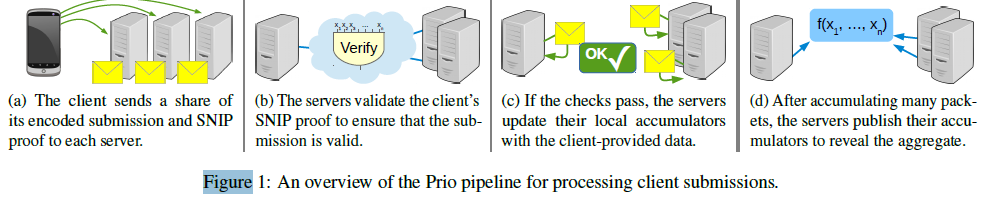
\includegraphics[scale=0.5]{img/prioPip.png}
\end{figure}

\subsection{Threat Model}
\textbf{Collective authority servers} In Prio, it is needed that all servers are not malicious and trusted so that security and privacy are guaranteed.\\
Robustness against malicious server seems desirable but that would impose an overhead in terms of cost privacy and performance degradation, which is not desirable.\\
Indeed if the sytem protects \textit{robustness} in the presence of $k$ faulty servers, it can protect \textit{privacy} only against a coalition of at most $s-k-1$ malicious servers. This is because $s-k$ honest server must be able to produce a correct aggregattion function even if $k$ faulty servers are offline. This is describe more formally in Prio original paper \cite{prio}, but increasing robustness weakens privacy in these conditions.\\
\textbf{Data providers} are assumed to be malicious. The system protects itself against malicious DPs. All data that do not pass the SNIPs proof, will be discarded.\\

\subsection{Pipeline and proof}
Prio's pipeline is a little different than Unlynx, as first the proof is ran on the data when they arrived and if they pass the proof, they are stored and aggregated later with more data.\\
First, it is needed to define an arithmetic circuit, $Valid(.)$, for each data provider.
When the data provider runs the circuit with its secret value $x$ as input, and sends a share $[x]_i$ of the secret value to server $i$, such that $\sum_{i}{[x]_i} = x $ along with a share of the polynomial $[h]_i$ derived from the circuit. The output of $Valid(x)$ is $1$.\\ 
This circuit is only defined in function of the number of bits of each share $[x]_i$ from the data provider, so it also sends a configuration file to the server such that it can reconstruct the circuit to verify the input. From this circuit, $3$ polynomials are extracted $f,g $ and $h$.\\

The data providers first upload their shares $[x_i]_1,...,[x_i]_m$ of their respective private value and a share of polynomial $h$ extracted from the arithmetic circuit.\\
The servers verify the SNIPs provided by the data providers to jointly confirm that $Valid(x_i) = 1$. If it fails, the server discards the submission.\\
Then each server saves in an accumulator the data they need to aggregate and they all together run the collective aggregation on the verified data.\\
When received inputs from all the involved DPs, they each publish their aggregation result to yield the final aggregation ( which is the sum of all aggregation ) result.

\subsection{Prio range validation (SNIPs)}
In this section, we describe into more details the secret-shared non-interactive proofs(SNIP) protocol.\\
\textit{Assumption}: A \textbf{Valid} circuit has $M$ multiplication gates, we work over a field $\mathbb{F}$ such that $ 2M << |\mathbb{F}| $\\
\subsubsection{Data provider evaluation}
First the data provider (DP) evaluates the circuit \textbf{Valid} on its input $x$. It constructs three polynomials $f,g $ which encode respectively the input wires and the ouput wire of each of the $M$ multiplication gates in the \textbf{Valid($x$)} circuit.\\
This step is done by polynomial interpolation to construct $f,g$ and get $h = f \cdot g$ .\\
So polynomials $f,g$ have a degree at most $M-1$ while $h = f \cdot g$ have a degree at most $2M-2$.\\
Then the DP splits the polynomial $h$ using additive secret sharing and sends the $i$th ($[h]_i$) share to server $i$.
\subsubsection{Consistency checking at the server}
At this time each server $i$ holds the shares $[x]_i$ and $[h]_i$ sent by the data provider. From both these values, the servers can reproduce $[f]_i$ and $[g]_i$ without communicating with each other.\\
Indeed $[x]_i$ is a share of the input, and $[h]_i$ contains a share of each wire value coming out of a multiplication gate. Thus, it can derive all other values via affine operations on the wire.
\subsubsection{Polynomial identity test}
Now each server has reconstructed shares $[\hat{f}]_i, [\hat{g}]_i$ from $[h]_i$ and $[x]_i$. It holds that $ \hat{f} \cdot \hat{g} = h$ if and only if the servers collectively hold a set of wire values that, when summed is equal to the internal wire value of the \textbf{Valid($x$)} circuit computation.\\
All execute the Schwartz-Zippel randomized polynomial identity test \cite{polyverif} to check if relation holds and no data have been corrupted or malicious DPs have tried to send wrong data.\\
The principle is that if $ \hat{f} \cdot \hat{g} \neq h$, then the polinomial $ \hat{f} \cdot \hat{g} - h$ is a non-zero polynomial of degree at most $2M-2$ in $\mathbb{F}$. It can have at most $2M-2$ zeros, so we choose a random $r \in \mathbb{F}$ and evaluate this polynomial, the servers will detect with probability at least $1 - \frac{2M-2}{|F|}$ that $ \hat{f} \cdot \hat{g} \neq h$.\\
The servers can use a linear operation to get share $\sigma_i = [ \hat{f}(r) \cdot \hat{g}(r) - h(r)]_i$. Then publish this $sigma_i$ to ensure that $\sum_{i}{\sigma_i} = 0 \in \mathbb{F}$. If it is not $0$ the servers reject the client submission.
\subsubsection{Multiplication of shares}
Finally all servers need to multiply the shares $ [\hat{f}(r)]_i $ and $ [\hat{g}(r)]_i$ to get the share $[\hat{f}(r)]_i \cdot [\hat{g}(r)]_i$ without leaking anything to each other about the values of the two polynomials. It is here that the Beaver MPC enters the computation. Each server also received from a trusted dealer one-time-use shares $([a]_i,[b]_i,[c]_i) \in \mathbb{F}^3 $ such that $a \cdot b = c \in \mathbb{F}$. We can from this shares, efficiently compute a multiparty multiplication of a pair of secret-shared values. This only requires each server to broadcast a single message.\\
The triple is generated by the data provider but it could be generated by the servers themselves by following an interactive secure protocol. There habe been a lot of works in this topic during the last years. This would avoid the dependency on the data provider to generate these values, which could lead to forging them to make the servers accept the test by designing alpha to cancel out the sum shown at the end of the paragraph.\\
The servers are then able to compute if values are correct. Moreover, even if the data provider sends wrong values, the server still catches the cheating data provider with high probability. Indeed if $a \cdot b \neq c \in \mathbb{F}$ then we can write $a \cdot b = (c + \alpha) \in \mathbb{F}$. We can then run the polynomial identity test with $\hat{f}(r) \cdot \hat{f}(r) - h(r) + \alpha = 0$. The servers will catch a wrong input with probability at least $1 - \frac{2M-2}{|F|}$.

\subsubsection{Output verification}
If all servers are honest, each will hold a set of shares of the \textbf{Valid} circuit's values. To confirm that \textbf{Valid($x$)} is indeed $1$ they only need to publish their share of the \textit{output wire}. Then, all server sum up to confirm that it's indeed equal to $1$, except with some small failure probability due to the polynomial identity test.


\section{Implementation}
This section details what was implemented more thoroughly. We include the description of the deployed code, but also of the theoretical work done to design some algorithms.
First, we will address the implementation of Prio:\\

Prio code \cite{priocode} was implemented in Go, with 3 dependencies in C (FLINT, GMP, and MPFR) to execute polynomial operations and designed by Henry Corrigan-Gibbs.\\
This project contribution is mostly porting code to use the multiparty computation and SNIPs in the Unlynx framework. So most of the code is used directly from the repository, but all the communication between the servers and with data providers has been reworked to be compatible with the Tree structure used in Unlynx \cite{unlynxcode}.\\
To follow the structure, the aggregation and verification protocols were split into two different protocols, even if they both work together to get the final result.\\
To be more precise, data provider sends shares $[x_i]$ and $[h_i]$, to the servers that do the SNIPs proof by evaluating the share on the \textit{Valid()} circuit, do the MPC to fuse each validation of the shares , if it passes it aggregates the result of the SNIPs, else it will discard.\\
Let's start by describing the easiest protocol, the aggregation and then the validation.\\
\subsubsection*{Aggregation}
The protocols are run at each server $j$, and each protocol has received a share $[x_i]_j$ from data provider $i$ represented by an array \textit{type big.Int} in Go. The protocol structure is a binary Tree.
This share actually represents the encoding in AFE of the original value which was an integer.\\

When several data have been received, aggregation starts by the root protocol, that notifies all children that the aggregation will start, and wait for the children to send their local sum. This notification goes down the Tree until there are no more children, and at this point each leaf $l$ aggregates locally the share by simply summing $\sum_{i}[x_i]_l$, and sends the result to their unique parents. On receiving the response from its children, the other nodes aggregate locally their own shares, and send to the parent. This is done until the root has received all the data. It then aggregates all the data and publishes them.\\
The only optimization made is the transfer of shares between server. The structure transforms these shares into a byte array and uses the method of big int to set it directly back from byte array to a big integer. This is made because the transfer functions are more efficient with bytes.\\

However, Prio has a more interesting feature that helps aggregating different types of data and doing different aggregation functions. Indeed, one can represent the value to aggregate with an AFE, where the AFE is an array of \textit{big.Int}. This helps computing OR and AND, MIN and MAX and even set intersection/union given only the aggregation of the special AFE encoding for each of this functions.\\
To illustrate an AFE, let's see the OR. To do OR($x_1,...x_n)$ where $x_i \in \{0,1\} $, $x$ is encoded as followed in $\mathbb{F}_2^{\lambda}$ (for a $\lambda$-bit string):
\begin{align*}
    Encode(x)=\left\{
                \begin{array}{ll}
                  \lambda		\text{                                          if x = 0}\\
                  \text{Random element} \in \mathbb{F}^{\lambda}_{2}		\text{											if x = 1}\\
                \end{array}
              \right.
\end{align*}
The Valid algorithm is always true as long as you have same size encoding. To Decode, we output 0 if and only if the $\lambda$-bit string is composed of $\lambda$ 0. This AFE outputs the boolean OR-private of the values with probability $p = 1- 2^{-\lambda}$, over the randomness of the encoding.

As seen previously, we can compute a function thanks to the sum of the AFE encoding. So the only modifications that have to be made on the input data and on the way the final result is computed at the root ( it's the Decode algorithm). No modification to the protocol should be made in order to compute different statistics.

\subsubsection*{Verification}
The verification protocol is the part where the multiparty computation is done. The data provider runs a function to create requests for the servers from 3 parameters: \textit{Its secret data, the number of servers, and the index of the leader for the request}.\\
This will create a request for each server, by creating a \textbf{Valid} circuit, evaluating the secret on it and constructing the polynomial. Each request contains a share of the Beaver MPC $[a]_i, [b]_i $ and $ [c]_i$, but more importantly, a share of the secret value $[x]_i$ and one of the polynomial created previously $[h]_i$.\\

The splitting is optimized by Prio, in a way that instead of picking the $s-1$ shares randomly and setting the last one, it uses a pseudo-random generator (such as AES in counter mode). You can then pick the keys and share them instead of sharing the integer directly.
Then the data provider sends to each server the request it is assigned to. From this point, before stepping into the proof, the protocol needs to initialize some parameters.\\

First, it will reconstruct the \textbf{Valid} circuit from the type and number of bits of the data provider data which are public.  Two structures called \textit{Checker} and \textit{CheckerPrecomp} were already implemented in the Prio code and are re-used from the original implementation. They are initialized with the circuit computed previously and the leader index. The leader is the server that returns the proof result, and that coordinates the proving protocol.
The protocol starts by assigning a request to the Checker structure and reconstituting the polynomial shares $[f]_i $ and $[g]_i$ for server $i$. It then evaluates the expression $[d]_i $ and $[e]_i$ from the MPC protocol described in \textbf{Background}. Then they all broadcast these shares, and reconstruct $d$ and $e$.
An optimization was also already done in Prio, which is the verification without interpolation. The point $r$ to do the polynomial test is fixed beforehand, this way any server can interpolate and evaluate in one single step.\\
Then the goal is to check that the evaluation of $\hat{f}(r) \cdot \hat{g}(r) -\hat{h}(r) = 0$ at each server. These values are all sent to the root that checks that the sum is 0.
In the same ways as before all communications are made in bytes, and channels are used to solve waiting for result problem.\\
At the end, the protocol returns the original shares to aggregate, that is the output of the circuit evaluate on shares, if the test is true, or empty shares if the protocol fails.


\subsubsection*{Input Range}
Now we're going to look at the input range validation implementation for EC ElGamal:\\

First and foremost, pairing over elliptic curve is not supported by all the curves So we used a pairing already implemented by DeDiS in the paper dfinity repository \cite{dfinitydedis}.  This is based on a Barreto-Naehrig curve implementation produced by dfinity \cite{dfinity}, that uses some libraries in C++ depicted in the GitHub description. We then use this curve for the whole Unlynx protocol. This is experimental, as security should be studied again with this new parameter.\\

Then, we need to prove to a single server that a secret $\sigma$ lies in a given range. 
The Range proof validation protocol assumes that the verifiers sign each element of the base $u$ with a key that has to remain secret. Indeed for the soundness of the protocol, i.e. if the statement is false no cheating prover can convince the honest verifier that it is true, except with a small probability, we don't want the prover to be able to forge signatures.
With Boneh-Boyen signature, as long as the key remains secret, this property holds.\\
For the Anytrust model considered here, we cannot make the computation of the key with a sequential protocol, as they will all have the same private key and if one divulgates it, the soundness of the protocol does not hold. \\
 The first one is the computation of signature in a sequential way (in the same way as the key switch protocol does), with each server having their own private key, and contributing to the final signature. Every step should be verified with zero-knowledge proof, and at the end, the final server broadcasts the signatures computed, and the public key constructed to verify those. This way, no server can leak the private key because it is not constructed, but all server have the same signatures. \\
The second one is that each server has its own private key and computes the signatures. All server will verify an input from a data provider and the protocol passes if and only if all server found that the secret $\sigma$ indeed lies in the given range. This ensures that at least one proof has been done on a secret key that remained secret.\\
The collective construction of signatures would be a better choice, but it needs the computation of an inverse collectively. Because of the uncertainty of this approach, the second approach was chosen.

\begin{algorithm}[H]
\caption{Non-Interactive Range Validation}\label{euclid}
\begin{algorithmic}[1]
\State \textbf{Common Input:} $B$ the base point in the EC, $P$ the public key used to encode data, $u, l$ 2 integers and commitment $C$.
\State \textbf{Prover Input:} $\sigma$ the secret integer mapped to a point and $r$ a scalar in the EC such that $C = \sigma + Pr$, $\sigma \in [0,u^l)$\\

\State \textbf{Initialization Phase}: Each server $i$ in the collective authority compute the following values :\\
Pick a random $x_i \in \mathbb{Z}_p$\\
$y_i \gets Bx_i$\\
$A_{i,j} \gets B(x_i + j)^{-1} $, $\forall i \in \mathbb{Z}_u$ and $j \in \{1,...,m\}$\\
\State  \textbf{Servers} make their signature public as well as the key $y_i$. When a query is issued by a querier $Q$, we now assume that the range are contained in the query and broadcasted by the server as usual to the data provider.\\

\State \textbf{Online Phase}: Data provider encodes the signature of the value to check in base $u$ with randomly picked $v_j$.\\
So $\forall j \in \mathbb{Z}_l $ such that $ \sigma = \sum_{j}{\sigma_j u^j}$, it picks $v_j \in \mathbb{Z}_p$ and compute $V_{i,j} = A_{i,\sigma_j}v_j$\\
It also picks 3 values $s_j,t_j,m_j \in \mathbb{Z}_p $, $\forall j \in \mathbb{Z}_l$ and sends:\\
First : a value $c = H(B,C,y_i)$, where $H()$ is a cryptographic hash function.\\  Then: $Z_r = m-rc$ and $D \gets \sum_{j}{(u^j s_j + Pm_j)}$\\
And eventually $ \forall j \in \mathbb{Z}_l$\\
$a_{i,j} \gets e(V_{i,j},B)(-s_j)+e(B,B)(t_j)$\\ $Z_{\sigma_j} \gets s_j-\sigma_j c$ and $Z_{v_j} \gets t_j-v_j c$\\
To be more precise the data provider sends the following values to ALL servers: $ c, Z_r, Z_{v_j}, Z_{\sigma_j}$ with $C$ the encrypted value public, and $D, a_{i,j}$ value published to check proof.\\

\State Server $i$ checks that $D = Cc + PZ_r + \sum_{j}{(u^j Z_{\sigma_j}}) $\\
$a_{i,j} = e(V_{i,j},y)c + e(V_{i,j},B)(-Z_{\sigma_j}) + e(B,B)(Z_{v_j})$, $\forall j \in \mathbb{Z}_l$ , and publish the result.\\

Then the server responsible for the data provider keeps the value if all the published value match the one computed by the data provider.
\end{algorithmic}
\end{algorithm}

At the end of the protocol, all values computed are made public so that anyone can verify that the servers have computed the verification correctly and act accordingly.\\

The completness follows from inspection. The soundness is still based on the Boneh signature.\\
The zero-knowledge was satisfied in the interactive version of this protocol. As we use the Fiat-Shamir heuristic \cite{fiatshamir} to transform the protocol into a  non-interactive one, the zero-knowledge property is still assumed to hold.\\

Let's now look at the communication complexity.
The initialization phase, which includes signature and public key sending, is not counted as a part of the protocol, as it is executed once in the beginning and reused afterwards.\\
The prover sends $l$ blinded values $V_j$ to each verifier, as well as $l$ $Z_{\sigma_j}$ and $Z_{v_j}$ but also each $a_j$ computed from the blinded signatures, a challenge $c$, a value $Z_r$, and a value $D$.\\
Taking back the mapping $e : G_1 \times G_1 \rightarrow G_T$.\\
It requires $l \cdot |G_1|$ communication to send $V_j$, $l \cdot |Z_p|$ communication for both $Z_{v_j}$ and $Z_{\sigma_j}$. $a_j$  needs $l \cdot |G_T|$ communication, and the unique items $c,Z_r $ and $D$ require respectively $ |Z_p|, |Z_p| $ and $|G_1|$.\\
The total communication required for the protocol is:\\
$Com(P,V) = l \cdot (|G_1| + 2 \cdot |Z_p| + |G_T|) + |G_1| + 2 \cdot |Z_p|$


\subsubsection*{Optimizations}
The input range implementation can be further optimized and we discuss the possible improvements in this sub-section as well as what was implemented in the actual framework.\\
First of all, the service implemented consists of 3 steps: Range verification, Aggregation, and Key switch. This is the best approximation of service to compare with the Prio verification and aggregation, with the least differences.\\
This service is in no case optimized, it serves as a comparison, so a lot of values are hardcoded such as the number of client submission to wait for before aggregation or the keys for encryption are chosen beforehand randomly.\\

One thing is that each server received a different structure containing all parameters to validate including $C, c, \{V\}, \{Z_v\} ,\{ Z_{\sigma}\}, D $ and $a$. We could improve the protocol to compute only once the $D$ and $Z_r$, and pick for a single value the same $m_j, t_j$ and $s_j$ at prover.\\
This would lead to a small reduction in computation time in prover side, and some bandwidth reduction for servers.

\section{Performance evaluation}

This section presents the time required for the 3 different systems described in the previous section to execute a request. All test were run on VMWare, Ubuntu64 bits v17.10, 6.1 GB RAM, 2 cores Intel I5-4590 @3.3Ghz.\\
For Prio, 64 bits inputs are used, while we use a range of $[0,16^{16})$ for Unlynx.\\
We evaluate the computation time in function of the number of servers, with 10 data providers (each having one data point), and the scaling with the number of data providers with 5 fixed servers.\\

Further in this section, we use the term \textit{trusted Unlynx}. 
It represents the Unlynx system with the exact same Threat Model as Prio, i.e, we need all the server to be trusted to ensure correctness. The range validation is slightly modified, as the prover (DP) only need to send the proof to the server responsible for the aggregation of its data. This reduces drastically the communication, and the computation time because the server can verify in parallel the data coming from one data provider. In this system, the DP only compute one proof from one set of signature and send it to a single server, which also reduces the computation time at the data provider.\\
The data are assumed to be evenly distributed to the server in this context.

\subsubsection{Scaling in number of data providers}
We first present a figure showing a graphic with linear axes. The first column presents Prio protocol, the second one Unlynx with the assumption that we trust all servers, and the last one is the original  Unlynx. The number of server is fixed to 5.
\begin{figure}[H]
\centering
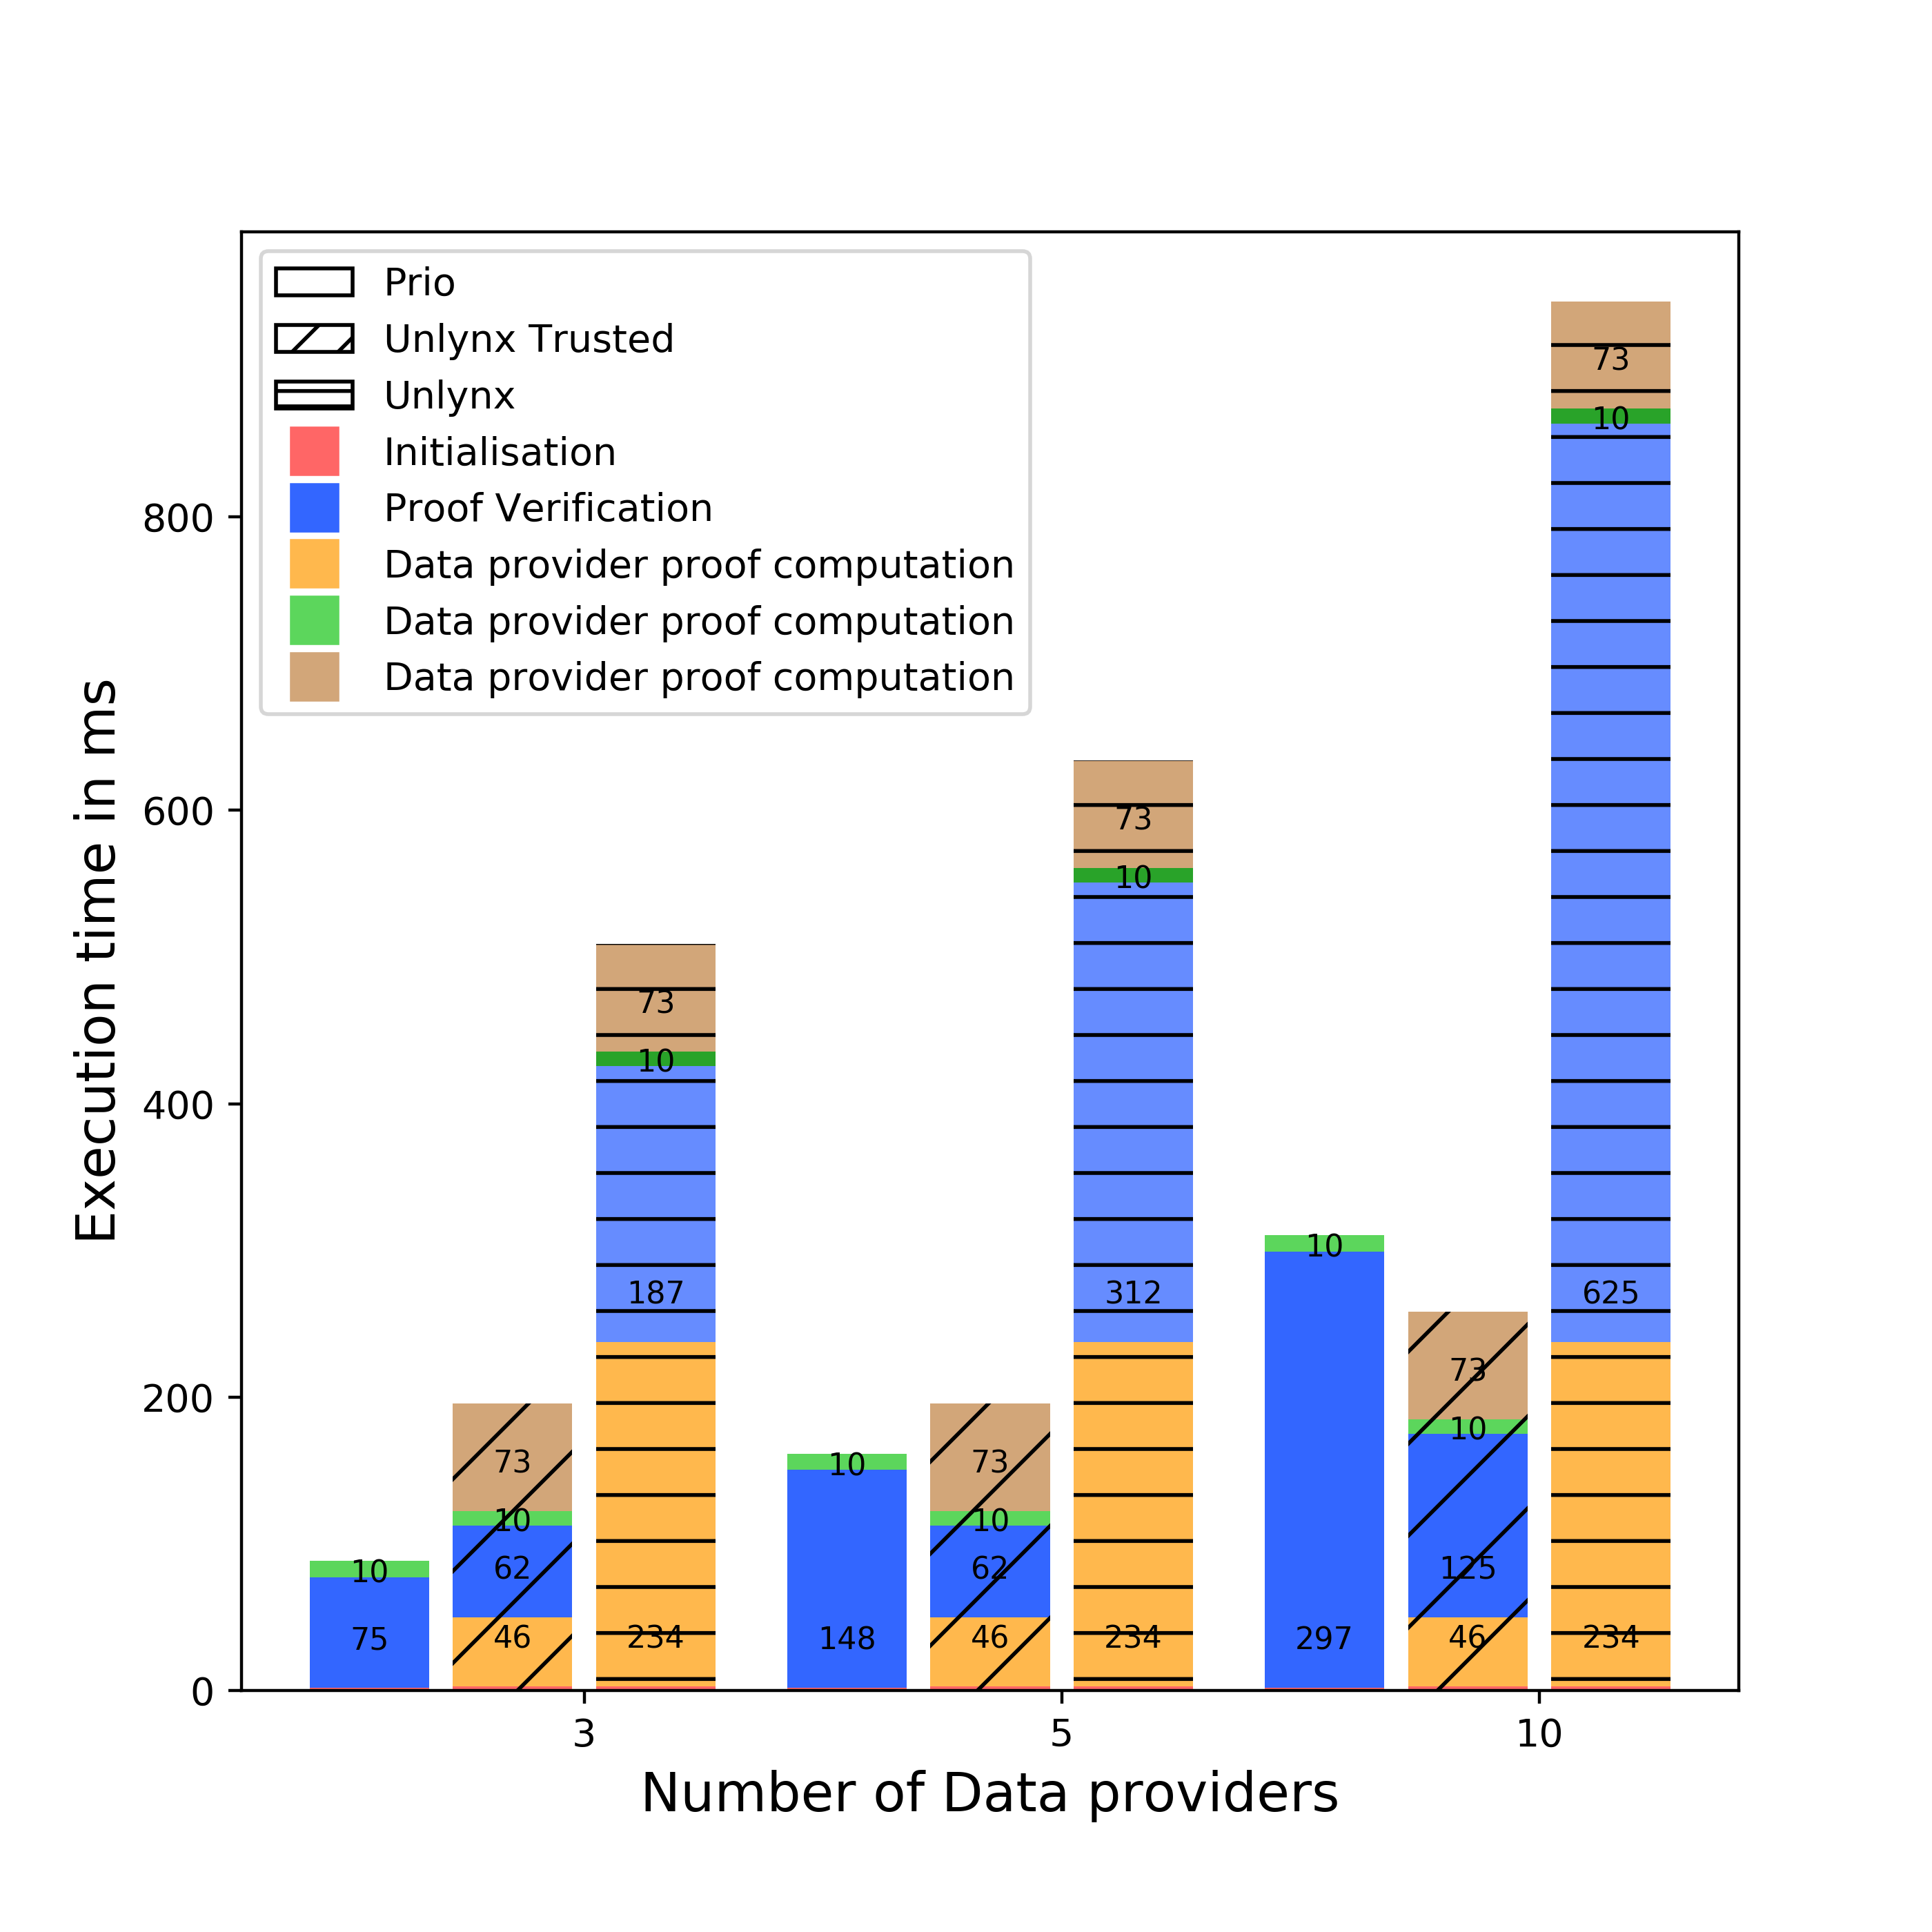
\includegraphics[scale=0.7]{img/ComparisonlinearDP.png}
\end{figure}
The comparison of computation time will be done in the same order as the protocol runs it.\\
First, an interesting computation time evolution to look at is the \textit{input validation}. In Prio, it grows linearly with a value of 75 ms at 3 servers and 297 ms at 10 servers. For the original Unlynx, it also grows linearly with the number of data providers, but starts at 187ms for 3 servers and hits 625 ms at 10 data providers. Trusted Unlynx beats both those systems with a linear growth in function of the ratio $\frac{\#DP}{\#Servers}$ (if the data are evenly distributed across all DPs). This leads to a time of 62ms for 3 and 5 servers, and 125 ms for 10 servers.
First, \textit{Initialization phases} for Prio or Unlynx are negligable compared to the other step of the protocol with an execution time inferior to 5 ms.\\
The \textit{Aggregation} protocol is constant for all protocol with an approximate time of 10 ms.\\
The difference of Threat model in the Unlynx protocol is accentuated with the DPs proof computation time. In the trusted one it is only 46 ms while in the non trusted, it is increase by a factor 5 (234 ms), which is the number of server.\\
Indeed in the second case the data provider need to compute the proof for each server.
At last, the \textit{Key Switch} protocol is constant with 73 ms no matter how many data providers there is.\\

Overall, when the number of data providers grows big enough, trusted Unlynx is the best protocol in front of Prio. The original Unlynx is way behin with an execution time almost 4 times superior to Prio.\\
We support our analysis with another figure, that scales the number of data providers to 500. The scale is of execution time is logarithmic, however, trusted Unlynx is the best protocol in term of execution time ahead of Prio, and both of them are way better than Original Unlynx.

\begin{figure}[H]
\centering
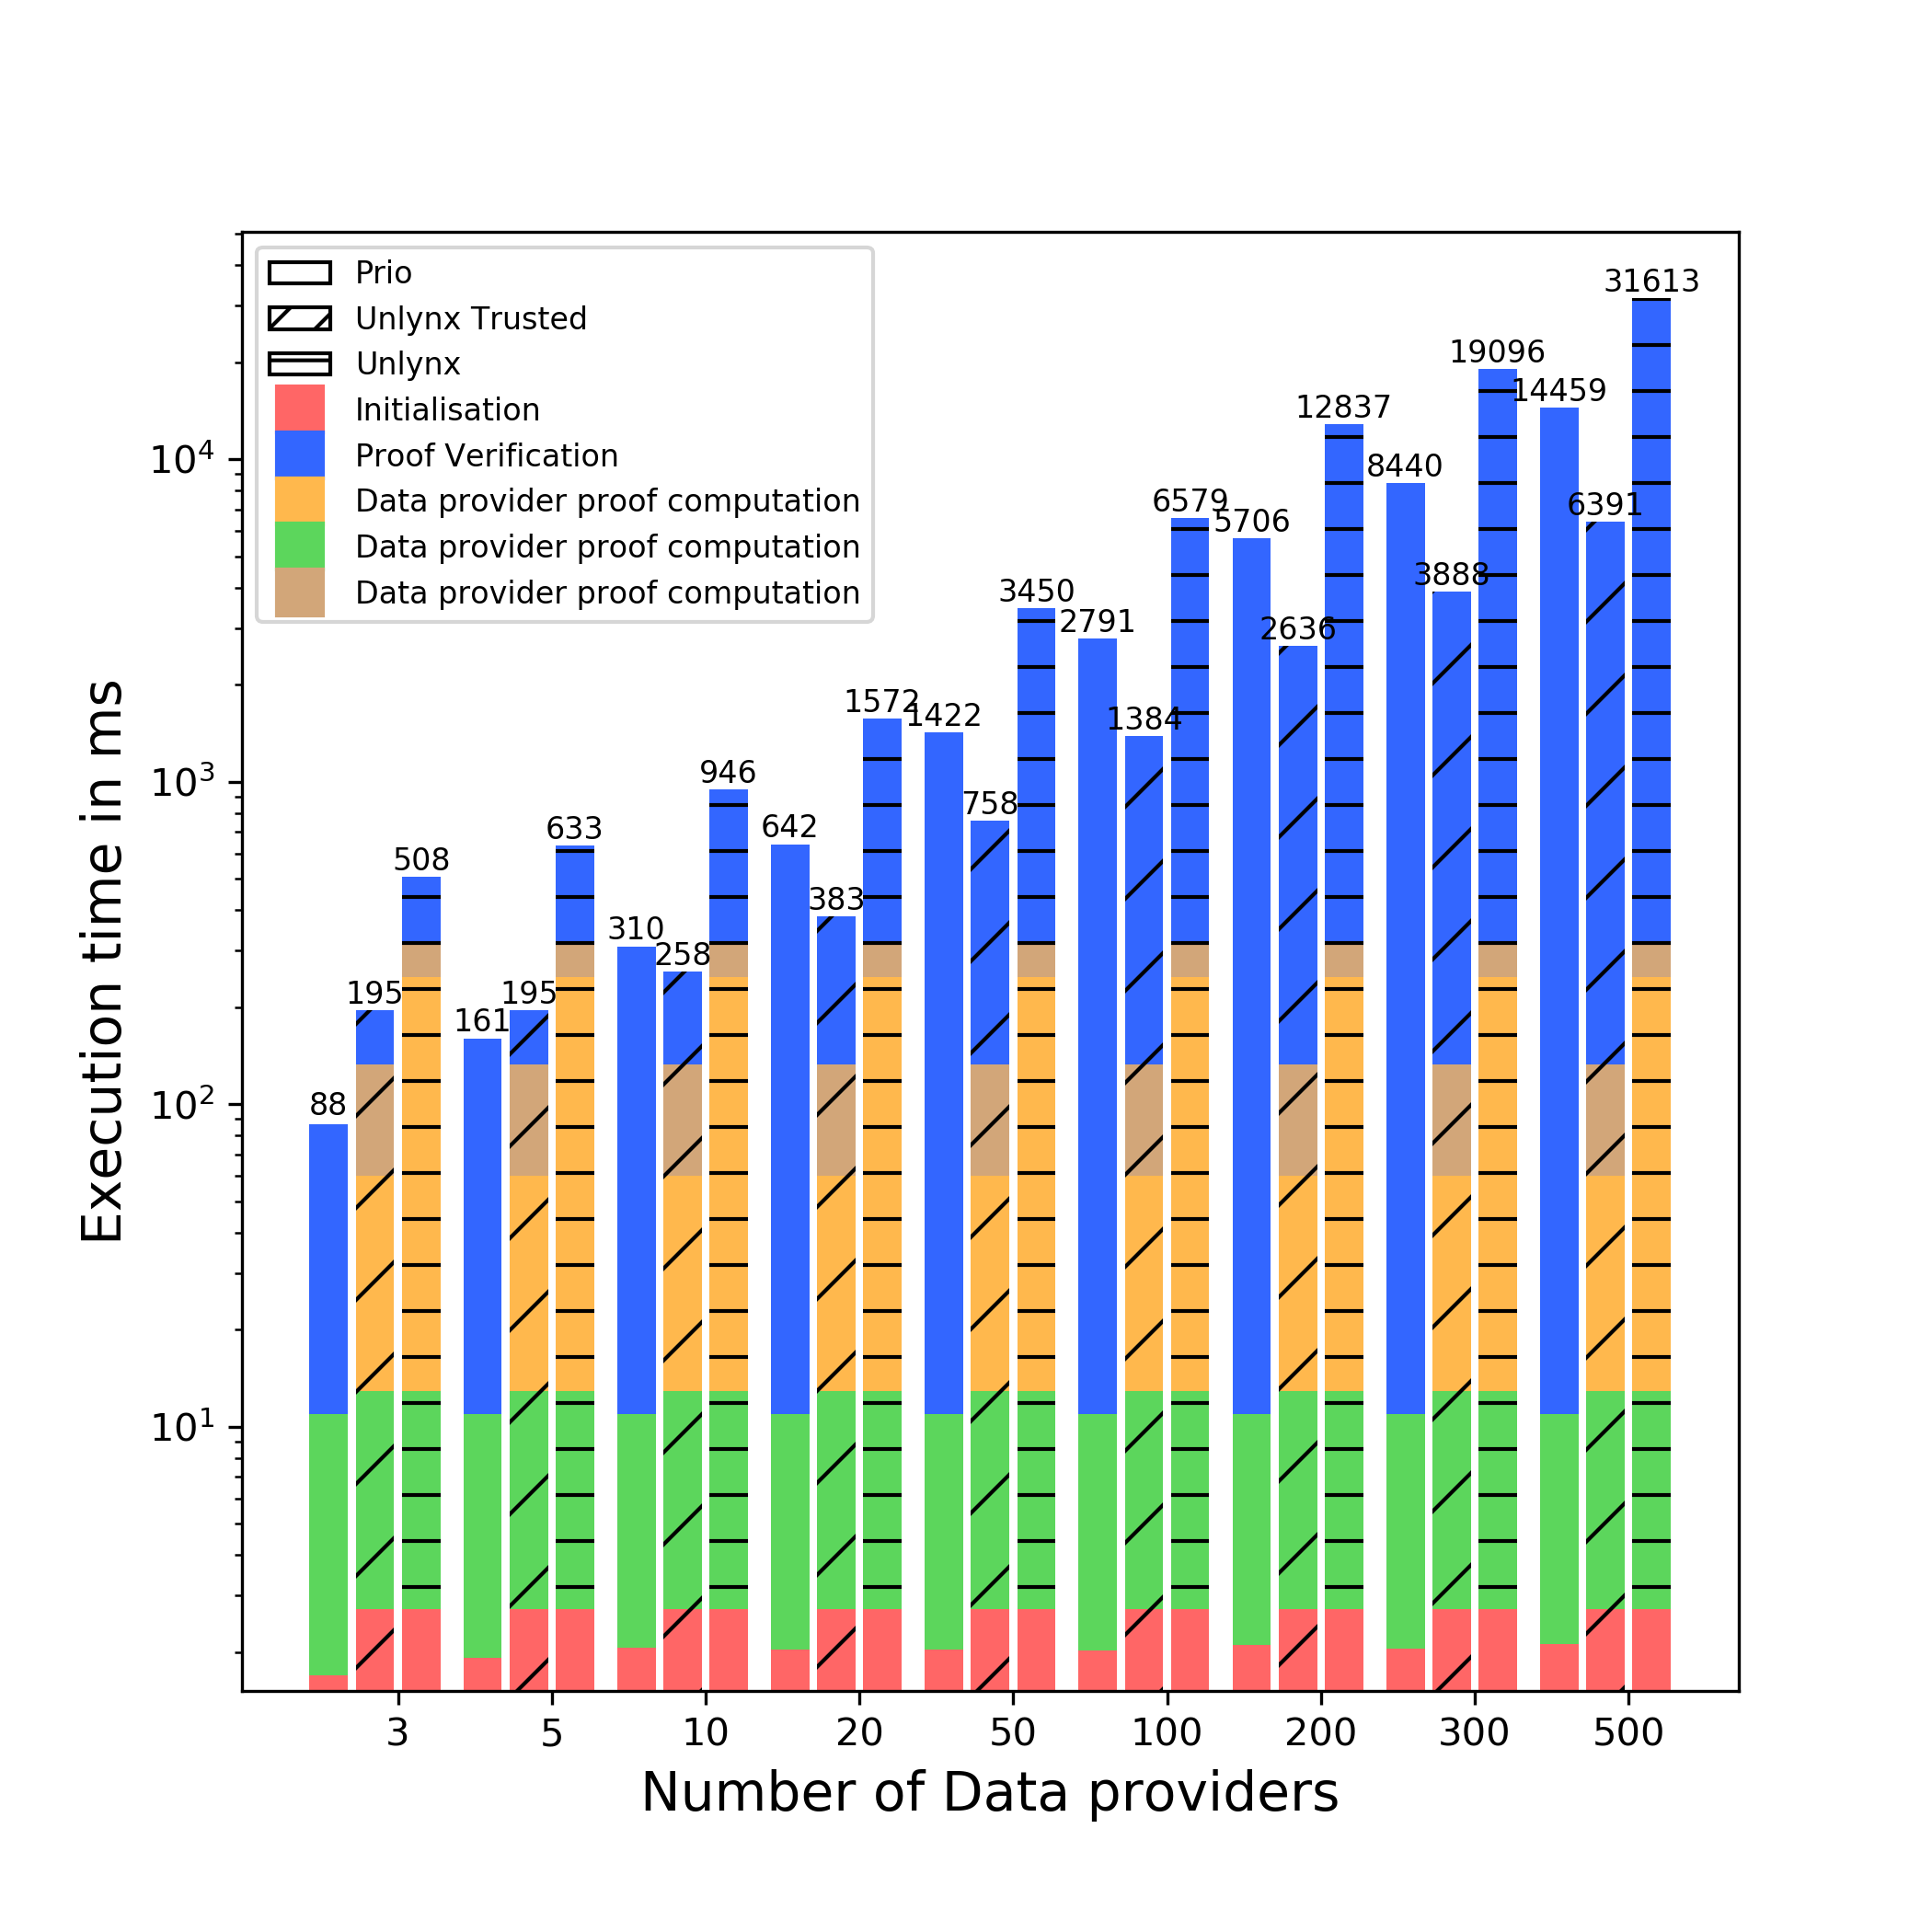
\includegraphics[scale=0.7]{img/ComparisonDP.png}
\end{figure}
 

\subsubsection{Scaling in number of data providers}

\begin{figure}[H]
\centering
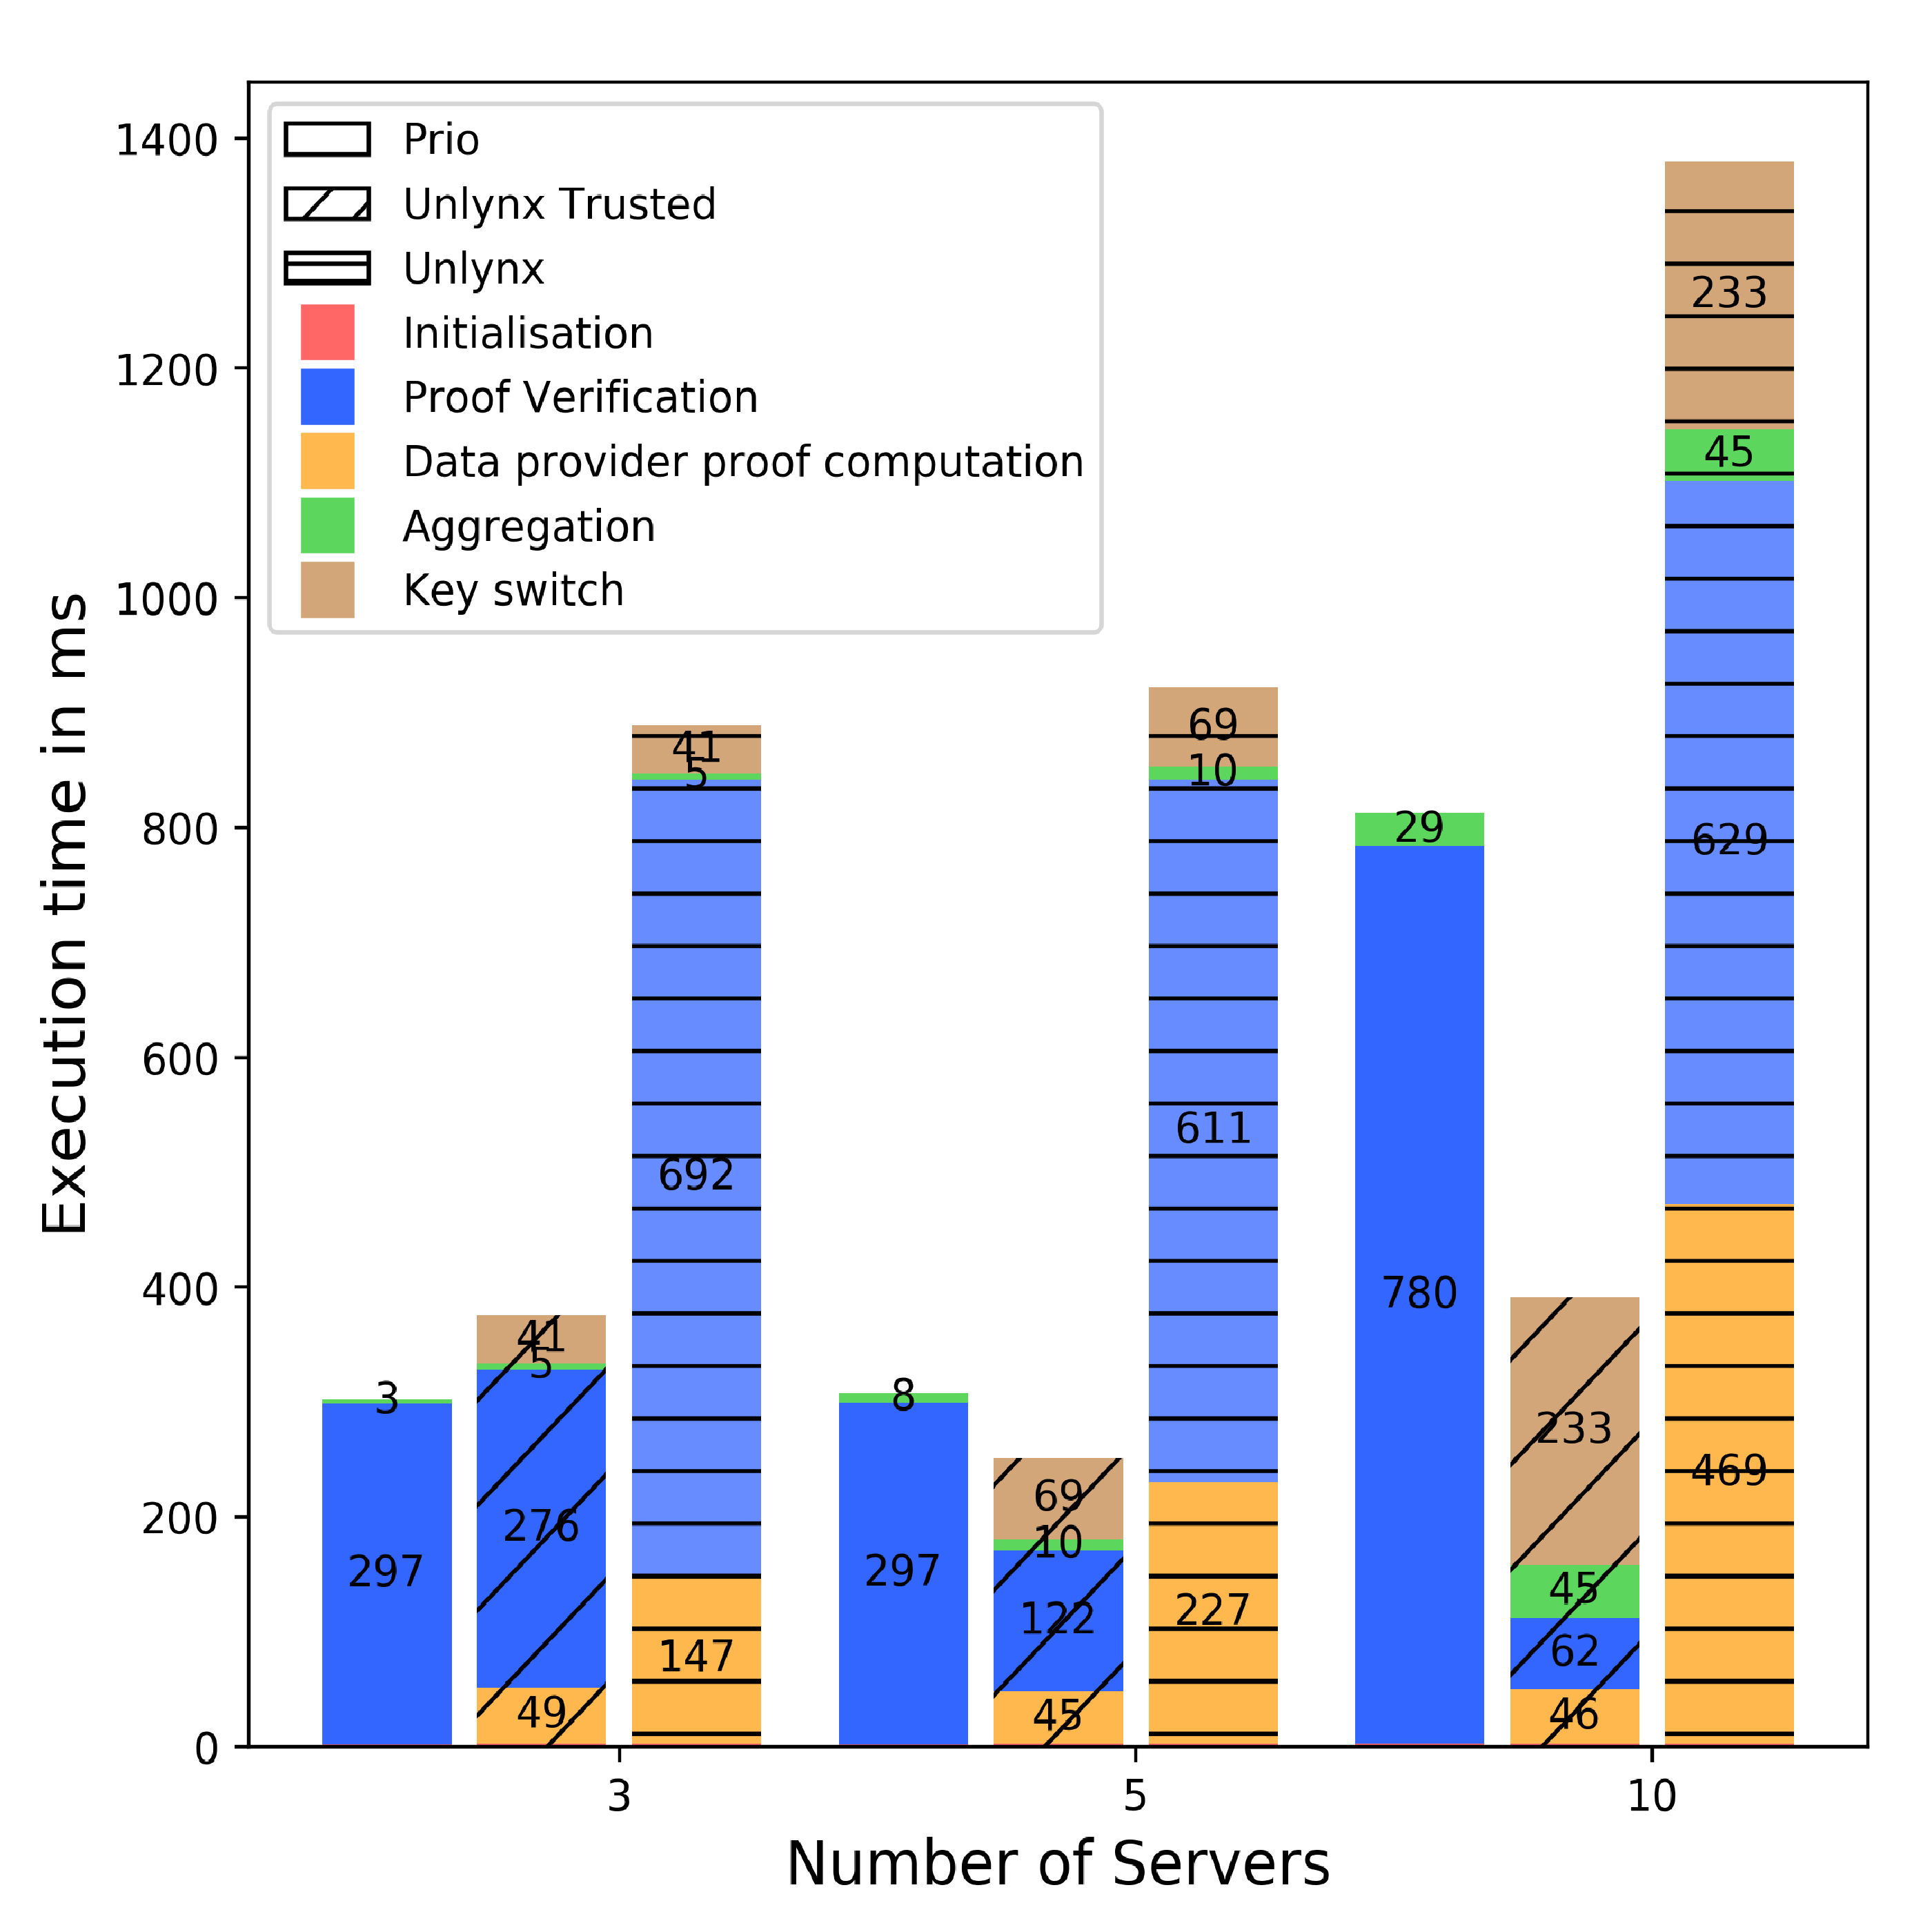
\includegraphics[scale=0.7]{img/ComparisonlinearServer.png}
\end{figure}

\begin{figure}[H]
\centering
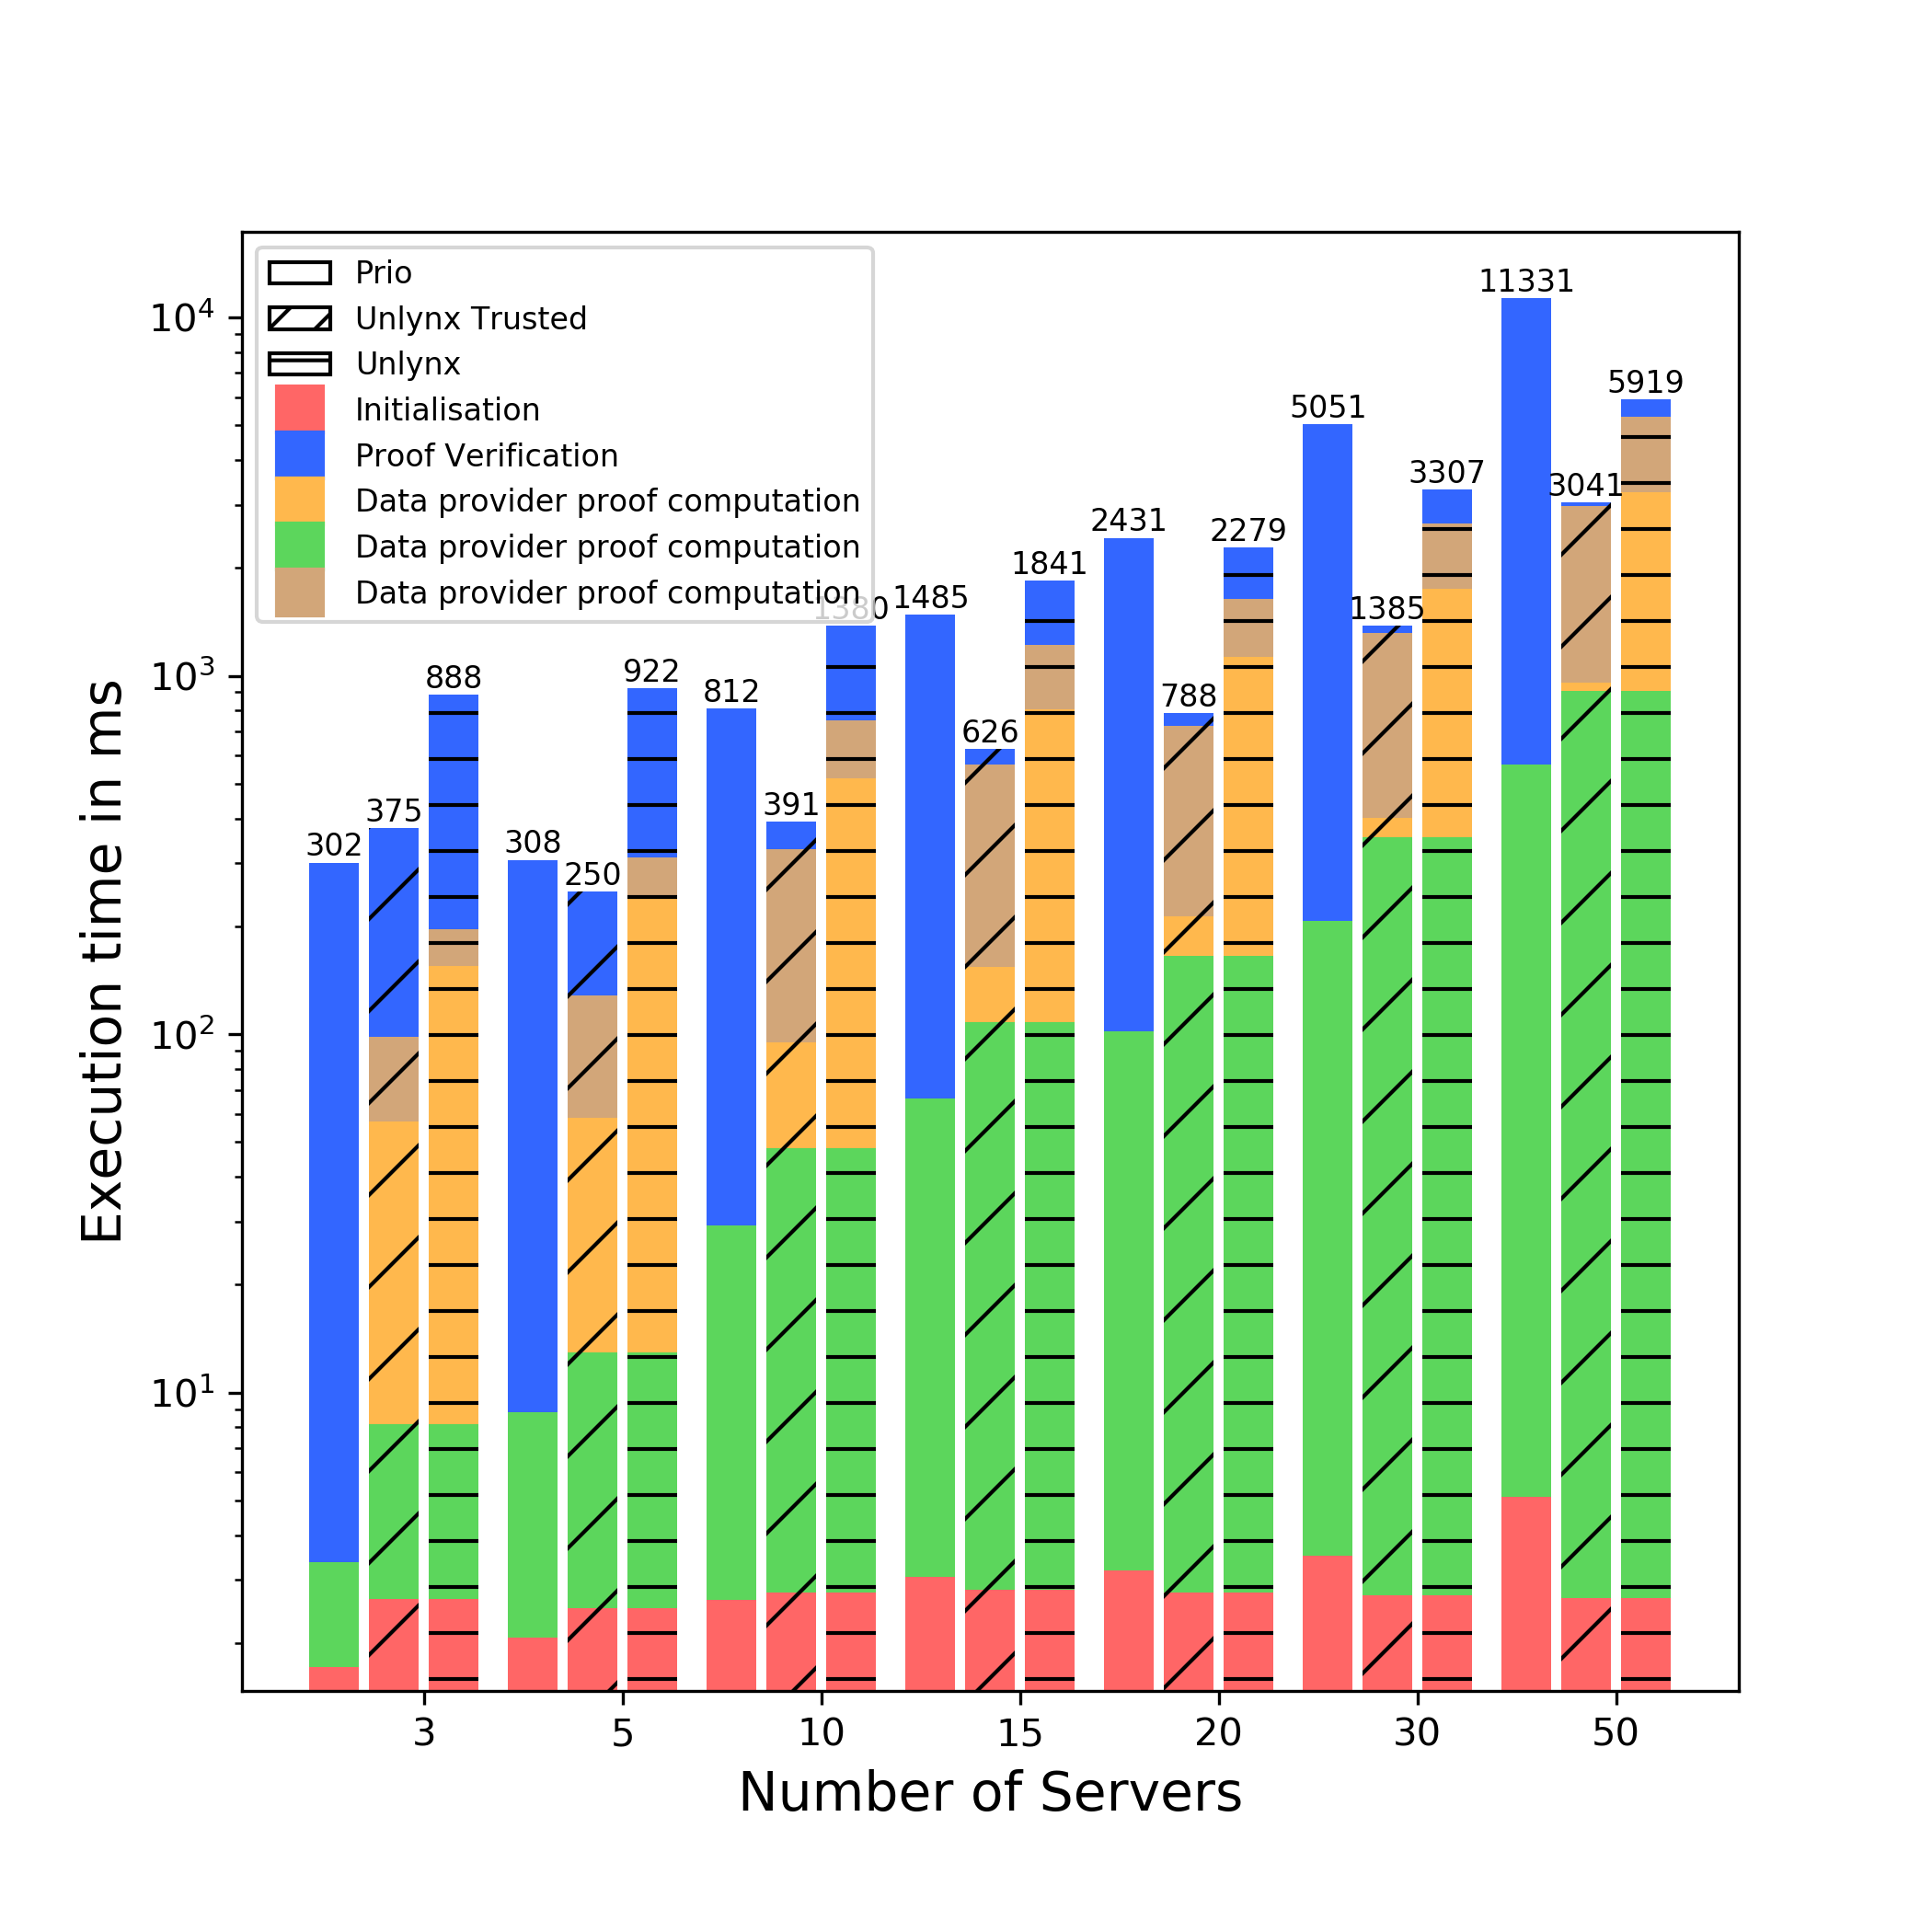
\includegraphics[scale=0.7]{img/ComparisonServer.png}
\end{figure}
\section{Systems' Comparison}
As explained previously, the service implemented for Unlynx range proof consists of 3 steps: Range verification, Aggregation, and Key switch. This is the best approximation of service to compare with the Prio verification and aggregation, with the least significant differences.\\
The key switch used is not the optimal one as it does not use the byte structure to communicate, due to a problem on the new Elliptic curve used.\\

The threat models are almost the same (the small difference is still in the collective authority, where you don't need to trust anyone for Unlynx) and we study the time it takes for an aggregation.\\
To be more precise in Prio, we measure the time, for different clients, it takes to verify all submissions, aggregate and publish the computed aggregate function.
While in Unlynx, the measured time is the sum of the verification, the aggregation of cipher and the key switch, as you need to turn back the aggregate data to readable data for the querier.\\

For Prio here is a table with some time and size measurement for 1 client input and different number of server:\\

\begin{table}[H]
\caption{Prio measurements}
\label{my-label}
\centering
\resizebox{\columnwidth}{!}{
\begin{tabular}{|
>{\columncolor[HTML]{656565}}c |c|c|c|}
\hline
{\color[HTML]{FFFFFF} \# Servers}                                                                                                                                                                    & \cellcolor[HTML]{656565}{\color[HTML]{FFFFFF} 3} & \cellcolor[HTML]{656565}{\color[HTML]{FFFFFF} 5}  & \cellcolor[HTML]{656565}{\color[HTML]{FFFFFF} 10} \\ \hline
{\color[HTML]{FFFFFF} \begin{tabular}[c]{@{}c@{}}Data provider initialization time ( creation of request for Prio protocol)\\ (6bits/32bits/64bits)\end{tabular}}                                    & 0.401 ms/ 1.83 ms / 3.45 ms                      & \multicolumn{1}{l|}{0.563 ms / 2.11 ms /3.329 ms} & \multicolumn{1}{l|}{0.863ms / 2.67 ms / 4.3 ms}   \\ \hline
{\color[HTML]{FFFFFF} \begin{tabular}[c]{@{}c@{}}Size of data sent in bytes by Data provider in function of circuit size\\ (136 bytes / 328 bytes / 584 bytes)\end{tabular}}                         & 136*3 / 328*3  / 584 *3                          & 136*5 / 328*5 / 584*5                             & 1360 / 3280 / 5840                                \\ \hline
{\color[HTML]{FFFFFF} \begin{tabular}[c]{@{}c@{}}Size of messages sent in broadcast phase of the protocol by 1 server\\ /Total size of all message exchanged in broadcast\\ (in bytes)\end{tabular}} & 32 / 96                                          & 64/320                                            & 144/1440                                          \\ \hline
{\color[HTML]{FFFFFF} \begin{tabular}[c]{@{}c@{}}Size of message sent by 1 server to root for final phase \\ / Total size of messages sent to root for final phase\\ (in bytes)\end{tabular}}        & 8 / 16                                           & 8 / 32                                            & 8 / 72                                            \\ \hline
{\color[HTML]{FFFFFF} \begin{tabular}[c]{@{}c@{}}Total time to execute the verification at the servers in function of circuit size\\ (6bits/32bits/64bits)\end{tabular}}                             & 8.07 ms/ 11.95 ms/ 19.57 ms                      & \multicolumn{1}{l|}{20.19ms / 35.95ms/ 46.80ms}   & \multicolumn{1}{l|}{67.85ms/85.72ms/115.1ms}      \\ \hline
{\color[HTML]{FFFFFF} \begin{tabular}[c]{@{}c@{}}Aggregation time for all server in function of data size in bits\\
(6/32/64)\end{tabular}}                                       & 2.32ms / 2.76ms / 3.1ms                   & 10.47ms / 11.06ms / 11.78ms                   & 29.37ms / 35.32ms / 37.93ms    \\ \hline          
\end{tabular}
}
\end{table}

We can state that the execution time grows linearly with circuit size, and it is mentionned in the paper that it is possible to do it with a sub-linear factor.\\ 
Moreover, the number of sent data is pretty low for small size data, and grows sub linearly with the size, in bits, of the data picked.\\

For Unlynx with range proof, assuming the same threat model as the orginal work we have the following:\\
\begin{table}[H]
\centering
\caption{Unlynx range proof measurement}
\label{my-label}
\resizebox{\columnwidth}{!}{
\begin{tabular}{|
>{\columncolor[HTML]{656565}}c |c|c|c|}
\hline
\multicolumn{1}{|l|}{\cellcolor[HTML]{656565}{\color[HTML]{FFFFFF} \# Server}}                                                                                     & \cellcolor[HTML]{656565}{\color[HTML]{FFFFFF} 3} & \cellcolor[HTML]{656565}{\color[HTML]{FFFFFF} 5} & \cellcolor[HTML]{656565}{\color[HTML]{FFFFFF} 10} \\ \hline
{\color[HTML]{FFFFFF} \begin{tabular}[c]{@{}c@{}}Time for initialization of Signature at 1 Server\\ in function of base u\\ (2/4/8)\end{tabular}}                  & 0.93ms/1.20ms/1.97ms                             & 0.93ms/1.20ms/1.97ms                             & 0.93ms/1.20ms/1.97ms                              \\ \hline
{\color[HTML]{FFFFFF} \begin{tabular}[c]{@{}c@{}}Size of Signature in function of base u at 1 Server\\ (2/4/8)\end{tabular}}                                       & 64 bytes /112 bytes /208 bytes                   & 64 bytes /112 bytes /208 bytes                   & 64 bytes /112 bytes /208 bytes                    \\ \hline
{\color[HTML]{FFFFFF} \begin{tabular}[c]{@{}c@{}}Time at Data provider to compute proof value\\ from signature in function of exponent l\\ (6/10/20)\end{tabular}} & 19.41*3 ms/31.75*3 ms/59.27*3 ms                          & 97.05ms/158.75ms/296.35ms                          & 194.1ms/317.5ms/592.7ms                           \\ \hline
{\color[HTML]{FFFFFF} \begin{tabular}[c]{@{}c@{}}Total size of message send by Data provider\\  to all server in function of l\\ (6/10/20)\end{tabular}}           & 1520 bytes/ 2480 bytes/ 4880 bytes               & 2480 bytes/ 4080 bytes/ 8080 bytes                 & 4880 bytes/ 8080 bytes/ 16080 bytes               \\ \hline
{\color[HTML]{FFFFFF} \begin{tabular}[c]{@{}c@{}}Computation time at 1 server for proof verification\\ in function of l\\ (6/10/20)\end{tabular}}                   & 25.02ms/39.16ms/81.18ms                          & 25.02ms/39.16ms/81.18ms                          & 25.02ms/39.16ms/81.18ms                           \\ \hline
{\color[HTML]{FFFFFF} Aggregation time}                                                                                                                            & 4.67ms                                           & 8.43ms                                           & 31.38ms                                           \\ \hline
{\color[HTML]{FFFFFF} Key switch time}                                                                                                                             & 19.34ms                                          & 37.97ms                                          & 97.28ms                                           \\ \hline
\end{tabular}
}
\end{table}
[TO FILL]


We also want to compare Prio and Unlynx with the exact same Threat Model, and in this case, the DP sends its data to the server it is connected to, and this server is the only one that does the verification of the proof for this DP. This solution gives us the following table:\\
\begin{table}[H]
\centering
\caption{Unlynx range proof measurement}
\label{my-label}
\resizebox{\columnwidth}{!}{
\begin{tabular}{|
>{\columncolor[HTML]{656565}}c |c|c|c|}
\hline
\multicolumn{1}{|l|}{\cellcolor[HTML]{656565}{\color[HTML]{FFFFFF} \# Server}}                                                                                     & \cellcolor[HTML]{656565}{\color[HTML]{FFFFFF} 3} & \cellcolor[HTML]{656565}{\color[HTML]{FFFFFF} 5} & \cellcolor[HTML]{656565}{\color[HTML]{FFFFFF} 10} \\ \hline
{\color[HTML]{FFFFFF} \begin{tabular}[c]{@{}c@{}}Time for initialization of Signature at 1 Server\\ in function of base u\\ (2/4/8)\end{tabular}}                  & 0.93ms/1.20ms/1.97ms                             & 0.93ms/1.20ms/1.97ms                             & 0.93ms/1.20ms/1.97ms                              \\ \hline
{\color[HTML]{FFFFFF} \begin{tabular}[c]{@{}c@{}}Size of Signature in function of base u at 1 Server\\ (2/4/8)\end{tabular}}                                       & 64 bytes /112 bytes /208 bytes                   & 64 bytes /112 bytes /208 bytes                   & 64 bytes /112 bytes /208 bytes                    \\ \hline
{\color[HTML]{FFFFFF} \begin{tabular}[c]{@{}c@{}}Time at Data provider to compute proof value\\ from signature in function of exponent l\\ (6/10/20)\end{tabular}} & 19.41ms/31.75ms/59.27ms                          & 19.41ms/31.75ms/59.27ms                          & 19.41ms/31.75ms/59.27ms                          \\ \hline
{\color[HTML]{FFFFFF} \begin{tabular}[c]{@{}c@{}}Total size of message send by Data provider\\  to its server in function of l\\ (6/10/20)\end{tabular}}           & 560 bytes/ 880 bytes/ 1680 bytes               & 560 bytes/ 880 bytes/ 1680 bytes                 & 560 bytes/ 880 bytes/ 1680 bytes               \\ \hline
{\color[HTML]{FFFFFF} \begin{tabular}[c]{@{}c@{}}Computation time at 1 server for proof verification\\ in function of l\\ (6/10/20)\end{tabular}}                   & 25.02ms/39.16ms/81.18ms                          & 25.02ms/39.16ms/81.18ms                          & 25.02ms/39.16ms/81.18ms                           \\ \hline
{\color[HTML]{FFFFFF} Aggregation time}                                                                                                                            & 4.67ms                                           & 8.43ms                                           & 31.38ms                                           \\ \hline
{\color[HTML]{FFFFFF} Key switch time}                                                                                                                             & 19.34ms                                          & 37.97ms                                          & 97.28ms                                           \\ \hline
\end{tabular}
}
\end{table}

[TO FILL]

\section{Future Work}
Depends on RESULT.

\newpage
\section*{Conclusion}
\addcontentsline{toc}{section}{Conclusion}
iufznfiozfoezizefez fze
fezfezfezfezfezfezf
ezfezfezfzefezfezfezfezfezfzefzefezfezfezfezfezfezfezfz

\newpage
\begin{thebibliography}{9}

\bibitem{unlynx} 
David Froelicher, Patricia Egger, João Sa Sousa, Jean Louis Raisaro, Zhicong Huang, Christian Mouchet, Bryan Ford and Jean-Pierre Hubaux.\\
\textit{UnLynx:} A Decentralized System for Privacy-Conscious Data Sharing. 
\textit{EPFL}
 
\bibitem{prio} 
Henry Corrigan-Gibbs and Dan Boneh.\\
\textit{Prio}: Private, Robust, and Scalable Computation of Aggregate Statistics.
\textit{Stanford University}


\bibitem{range} 
Jan Camenisch, Rafik Chaabouni, and abhi shelat\\
Efficient Protocols for Set Membership and Range Proofs.
\textit{IBM Research, EPFL, U. of Virginia}

\bibitem{expose}
Josh Keller, K.K Rebbeca and Nicole Pelroth\\
How many times has your personal information been exposed to hackers ?
\\\texttt{http://www.nytimes.com/interactives/2015/07/29technology/personaltech/what-parts-of-your-information-have-been-exposed-to-hackers-quiz.html}

\bibitem{pentagon}
Classified Pentagon data leaked on the public cloud, BBC news
\\\texttt{http://www.bbc.com/news/technology-42166004}

\bibitem{apple}
Andy Greenberg, Apple's 'differential privacy' is about colleccting your data-but not your data.
\\\texttt{https://www.wired.com/2016/06/apples-differential-privacy-collection-data/}

\bibitem{swiss}
Departement federal de l'economie, de la formation et de la recherche DEFR.
\\\texttt{https://www.amstat.ch}

\bibitem{lca}
LCA1 laboratory, EPFL.
\\\texttt{http://lca.epfl.ch/}

\bibitem{dedis}
DeDis laboratory, EPFL.
\\\texttt{https://dedis.epfl.ch/}

\bibitem{randomized}
Stanley L. Warner\\
Randomized response: A survey technique for eliminating evasive bias.\\
\textit{Journal of the American Statistical Association 60,309 (1965),63-69}

\bibitem{sold}
Ben Smith\\
Uber executive suggest digging up dirt on journalits.
\\\texttt{http://www.buzzfeed.com/bensmith/uber-executive-suggests-digging-up-dirt-on-journalists}

\bibitem{dyadic}
Dyadic security \texttt{https://www.dyadicsec.com/}

\bibitem{centralized}
Dan Bogdanov, Sven Laur, and Jan Wilemson.\\
\textit{Sharemind}: A framework for fast privacy-preserving computations. In \textit{European Symposium on Research in Computer Security}

\bibitem{anytrust}
David I Wolinsky, Hery Corrigan-Gibbs, Bryan Ford, and Aaron Jonhson.\\
Scalable anonymous group communication in the anytrust model. In \textit{5th European Workshop on System Security. 2012}


\bibitem{priocode}
Prototype implementation of Prio in Go
\\\texttt{https://github.com/henrycg/prio}

\bibitem{unlynxcode}
Decentralized privacy-preserving data sharing tool : Unlynx\\
\texttt{https://github.com/lca1/unlynx}

\bibitem{sell}
The business of Data selling\\
\begingroup
\fontsize{8pt}{10pt}
\texttt{https://www.theguardian.com/technology/2017/jan/10/medical-data-multibillion-dollar-business-report-warns}
\endgroup

\bibitem{law}
Law on Data protection in the United-States\\
\begingroup
\fontsize{8pt}{10pt}
\texttt{https://content.next.westlaw.com/Document/I02064fbd1cb611e38578f7ccc38dcbee/View/FullText.html?contextData=(sc.Default)\& transitionType=Default\& firstPage=true\& bhcp=1}
\endgroup


\bibitem{bitcoin}
Satoshi Nakamoto, Bitcoin: A Peer-to-Peer Electronic Cash System.\\
\texttt{https://bitcoin.org/bitcoin.pdf}

\bibitem{proof1}
C Andrew Neff. Verifiable mixing (shuffling) of ElGamal pairs (2004)

\bibitem{proof2}
C Andrew Neff. A verificable secret shuffle and its application to e-voting. In \textit{Proceedings ACM-CCS 2001}, pages 116--125, 2001.

\bibitem{boneh}
Dan Boneh and Xavier Boyen. Short signatures without random oracles. In christian Caching and Jan Camenisch, editors, EUROCRYPT, volume 3027 of \textit{Lecture notes in Computer Science}, pages 56-73. Springer,2004.

\bibitem{polyverif}
J. T.,Schwartz Fast probabilistic algorithms for verification of polynomial identities. \textit{Journal of the ACM} 27,4 (1980), 701-717.


\bibitem{dfinitydedis}
Paper on dfinity to do DKG with pairing.
\texttt{https://github.com/dedis/paper\_17\_dfinity}

\bibitem{dfinity}
dfinity Github repository
\texttt{https://github.com/dfinity/go-dfinity-crypto}

\bibitem{fiatshamir}
Fiat-Shamir heuristic to transform interactive proof of knowledge to non-interactive.
\texttt{https://en.wikipedia.org/wiki/Fiat\%E2\%80\%93Shamir\_heuristic}
\end{thebibliography}


\end{document}
